\documentclass[preprint,12pt]{elsarticle}
\biboptions{numbers,sort&compress}

\usepackage{amsmath,amssymb,amsfonts,bm}
\usepackage{mathtools}
\usepackage{graphicx}
\usepackage{booktabs}
\usepackage{hyperref}
\usepackage{xcolor}
\usepackage[protrusion=true,expansion=false]{microtype}
\usepackage{subcaption}
\usepackage{array}
\usepackage{multirow}

\DeclareMathOperator{\tr}{tr}
\DeclareMathOperator{\cond}{cond}
\DeclareMathOperator{\rank}{rank}
\DeclareMathOperator{\diag}{diag}

\hypersetup{
    colorlinks=true,
    linkcolor=blue,
    citecolor=blue,
    urlcolor=blue
}

\journal{International Journal of Heat and Mass Transfer}

% Allow the line breaker extra freedom so that long inline expressions in narrow
% measure do not produce overfull boxes.
\emergencystretch=3em
\hyphenpenalty=1000

\begin{document}

\begin{frontmatter}

\title{Invariance of the Guyer--Krumhansl Fourier-Resonance Sensitivity Singularity to Boundary Heat Loss in Laser Flash Testing}

\author[gu]{Vipin Gupta\texorpdfstring{\corref{cor1}}{}}
\ead{vipin.gupta@gurugramuniversity.ac.in}
\cortext[cor1]{Corresponding author.}

\affiliation[gu]{organization={Department of Mathematics, Gurugram University},
            city={Gurugram},
            state={Haryana},
            postcode={122018},
            country={India}}

\begin{abstract}
This paper studies whether boundary heat loss can remove the Guyer--Krumhansl (GK) parameter-identifiability singularity that arises in laser flash testing at the Fourier-resonance condition $B \equiv \kappa^2 / (\alpha_0 \tau_q) = 1$, where the sensitivity collinearity $\partial \theta / \partial \tau_q = -\partial \theta / \partial \kappa^2$ makes the Fisher Information Matrix (FIM) structurally singular. We derive the closed-form transfer function for the 1D GK system with asymmetric Robin boundary heat loss and prove (Theorem~1) that at $B = 1$ both the bulk propagation factor and the dynamic surface thermal conductivity collapse to their classical Fourier counterparts, so the GK temperature field coincides identically with the Fourier solution for all positions, all times, and all non-negative Biot numbers. The collinearity, the FIM null direction, and $\sigma_3 \equiv 0$ are therefore invariant under linear Robin cooling. Near resonance, the smallest singular value scales two-sided linearly as $\sigma_{\min} \propto |B-1|$, and a three-parameter Cramér--Rao bound analysis for $\bm{p} = (\tau_q, \kappa^2, Bi)^\top$ quantifies the practical precision corridor. Boundary dissipation and multi-sensor detection improve off-resonance precision but cannot resolve the exact singularity within the linear model class, with direct consequences for heat-loss-corrected flash data reduction.
\end{abstract}

\begin{keyword}
Guyer--Krumhansl heat conduction \sep Laser flash method \sep Boundary heat loss \sep Parameter identifiability \sep Fourier resonance \sep Fisher information matrix
\end{keyword}

\end{frontmatter}

\section*{Nomenclature}
\begin{table*}[h!]
\resizebox{\textwidth}{!}{
\begin{tabular}{llll}
\multicolumn{2}{l}{\textbf{Roman symbols}} & \multicolumn{2}{l}{\textbf{Greek symbols}} \\
$B$ & Dimensionless parameter ratio, $\kappa^2 / (\alpha_0 \tau_q)$ & $\alpha_0$ & Thermal diffusivity [$\mathrm{m^2 \cdot s^{-1}}$] \\
$Bi, Bi_0, Bi_L$ & Biot numbers at boundaries & $\delta$ & Near-resonance perturbation, $B - 1$ \\
$c$ & Volumetric heat capacity [$\mathrm{J \cdot m^{-3} \cdot K^{-1}}$] & $\epsilon$ & Constitutive perturbation parameter, $\max(\tau_q, \kappa^2)$ \\
$\bm{F}$ & Fisher Information Matrix & $\varepsilon$ & Surface emissivity \\
$h, h_0, h_L$ & Heat transfer coefficients [$\mathrm{W \cdot m^{-2} \cdot K^{-1}}$] & $\theta$ & Dimensionless temperature rise \\
$\bm{J}$ & Sensitivity Jacobian matrix & $\kappa$ & Non-local mean free path length [$\mathrm{m}$] \\
$L$ & Specimen thickness [$\mathrm{m}$] & $\kappa^2$ & Non-local spatial parameter [$\mathrm{m^2}$] \\
$m(s)$ & Bulk propagation factor in Laplace domain & $\lambda_0$ & Thermal conductivity [$\mathrm{W \cdot m^{-1} \cdot K^{-1}}$] \\
$\bm{n}$ & Outward unit normal vector & $\lambda_{\mathrm{eff}}(s)$ & Operational dynamic thermal conductivity \\
$N_t$ & Number of temporal measurement points & $\mu(s) = \lambda_{\mathrm{eff}}(s)/\lambda_0$ & Operational surface conductivity factor \\
$N_x$ & Number of spatial grid intervals & $\rho$ & Parameter sensitivity correlation coefficient \\
$\bm{q}, q$ & Heat flux [$\mathrm{W \cdot m^{-2}}$] & $\sigma_i$ & $i$-th singular value of sensitivity Jacobian \\
$s$ & Complex Laplace transform frequency [$\mathrm{s^{-1}}$] & $\sigma_n$ & Measurement noise standard deviation \\
$T, T_0$ & Temperature, initial/ambient temperature [$\mathrm{K}$] & $\sigma_{\mathrm{SB}}$ & Stefan--Boltzmann constant [$\mathrm{W \cdot m^{-2} \cdot K^{-4}}$] \\
$t$ & Dimensionless time & $\tau_q$ & Thermal relaxation time [$\mathrm{s}$] \\
$x$ & Dimensionless spatial coordinate along slab thickness & $\tau_N, \tau_R$ & Normal and resistive phonon relaxation times [$\mathrm{s}$] \\
$\Delta(s)$ & Characteristic denominator of transfer function & $\tau_\Delta$ & Dimensionless pulse duration, $\alpha_0 t_p / L^2$ \\
$t_p$ & Laser pulse duration [$\mathrm{s}$] & $\Lambda$ & Carrier mean free path [$\mathrm{m}$] \\
$\bm{V}$ & Right singular-vector matrix of $\bm{J}$ & $\eta$ & Relative accuracy threshold, $\operatorname{SE}(\hat{\tau}_q)/\tau_{q,0}$ \\
$C(Bi)$ & Near-resonance scaling prefactor & $C_{\mathrm{eff}}$ & Effective multi-sensor sensitivity coefficient \\
$R_J$ & Normalized collinearity residual norm & $C_{\mathrm{asymp}}$ & Asymptotic Fourier-limit prefactor \\
$\bm{c}$ & Estimable-functional coefficient vector & $\bm{g}$ & Near-resonance collinearity-defect amplitude \\
\multicolumn{2}{l}{\textbf{Subscripts / Superscripts}} & \multicolumn{2}{l}{\textbf{Acronyms}} \\
$0$ & Front surface ($x = 0$) or baseline property & BDF & Backward Differentiation Formula \\
$L$ & Rear surface ($x = 1$) & CRLB & Cramér--Rao Lower Bound \\
$\mathrm{conv}$ & Convective heat transfer & DPL & Dual-Phase-Lag \\
$\mathrm{rad}$ & Radiative heat transfer & FIM & Fisher Information Matrix \\
$\mathrm{crit}$ & Critical threshold value & FVM & Finite Volume Method \\
$\mathrm{laser}$ & Incident laser irradiation & GK & Guyer--Krumhansl \\
$\mathrm{null}$ & Null space direction & SVD & Singular Value Decomposition \\
\end{tabular}
}
\end{table*}


\section{Introduction}

The laser flash method, originally introduced by Parker et al.~\cite{parker1961flash} and codified internationally in ASTM E1461-13(2022)~\cite{astm2022standard}, is an established photothermal technique for determining the thermal diffusivity and thermal conductivity of solid materials. In a typical measurement, a short radiant energy pulse irradiates the planar front face of a small disc-shaped sample, and an infrared detector records the resulting transient temperature rise on the opposite rear face. In the classical adiabatic formulation, thermal diffusivity $\alpha_0 = \lambda_0 / (\rho c)$ is calculated directly from the half-rise time $t_{1/2}$ of the rear thermogram under the assumption of one-dimensional diffusive transport~\cite{parker1961flash}. Over several decades, the technique has found extensive use across aerospace engineering, nuclear materials, semiconductors, and thermal barrier coatings, covering temperatures from cryogenic levels to above 2500~K~\cite{blumm2025laser,vozar2004flash}. Continuous improvements in laser beam homogenization, optical pyrometry, and numerical parameter estimation have brought measurement uncertainties in standard materials down to sub-percent levels~\cite{blumm2002improvement}.

Despite its widespread success, the classical interpretation of laser flash measurements is based on Fourier's law of heat conduction, $\bm{q} = -\lambda_0 \nabla T$, which implies that thermal disturbances travel at infinite speed. To address this non-physical characteristic, Cattaneo~\cite{cattaneo1958forme} and Vernotte~\cite{vernotte1958paradoxes} introduced a finite relaxation time $\tau_q$, which describes thermal inertia through a hyperbolic wave equation. In modern contexts involving ultrafast laser heating, high-frequency microelectronics, cryogenic single crystals, and nanostructured materials, thermal transport can depart markedly from classical diffusion~\cite{cahill2003nanoscale}. When the specimen dimensions or thermal gradient lengths approach the carrier mean free path (MFP) $\Lambda$ or relaxation timescale, non-equilibrium and quasiballistic transport processes emerge~\cite{chen2001ballistic}. Under these conditions, boundary and interface scattering reduce the effective thermal conductivity, and local temperature gradients alone no longer dictate the heat flux~\cite{alvarez2007memory,guo2015phonon}.

To link microscopic phonon kinetics with continuum mechanics, Guyer and Krumhansl~\cite{guyer1966solution,guyer1966thermal} solved the linearized phonon Boltzmann equation for dielectric crystals in the hydrodynamic regime, where momentum-conserving normal scattering ($N$-processes) dominates over momentum-destroying resistive scattering ($R$-processes). Their formulation produced the continuum constitutive relation:
\begin{equation}
\tau_q \frac{\partial \bm{q}}{\partial t} + \bm{q} + \lambda_0 \nabla T - \kappa^2 \nabla^2 \bm{q} = \bm{0},
\label{eq:gk_dimensional}
\end{equation}
which supplements the Maxwell--Cattaneo--Vernotte equation with a nonlocal spatial Laplacian of the heat flux vector. Here $\tau_q$ denotes the relaxation time for resistive processes, and $\kappa^2 \sim \ell^2 = \frac{1}{5} v_s^2 \tau_N \tau_R$ is a nonlocal mean-free-path square parameter associated with normal phonon collisions. The Guyer--Krumhansl equation provides a continuum description of phonon hydrodynamics, predicting both Poiseuille-like collective phonon flow and wave-like temperature propagation, termed ``second sound''~\cite{guyer1966thermal,chester1963second}. While second sound was once observed only in cryogenic crystals such as solid $^4\mathrm{He}$, $^3\mathrm{He}$, Bi, and NaF, experimental studies have reported second sound and hydrodynamic phonon transport in graphite at temperatures exceeding 100~K~\cite{huberman2019observation} and even above 200~K~\cite{ding2022observation}. Extended irreversible thermodynamics and non-equilibrium thermodynamic frameworks have verified that the Guyer--Krumhansl relation satisfies non-negative entropy production~\cite{jou2010extended,cimmelli2009different,sellitto2016mesoscopic}.

Beyond cryogenic crystals and nanostructures, generalized non-Fourier heat conduction with Guyer--Krumhansl characteristics has been observed at room temperature in macroscopically heterogeneous and porous materials, such as biological tissues, rocks, and metal foams~\cite{both2016deviation,van2017guyer}. In these materials, internal interfaces, pore structures, and distributed thermal impedances generate effective macroscopic memory and spatial nonlocality resembling hydrodynamic phonon transport. In response to these findings, several analytical and numerical solutions for the Guyer--Krumhansl system have been developed. Kov{\'a}cs~\cite{kovacs2018analytic} obtained an analytical Laplace-domain solution for 1D Guyer--Krumhansl heat conduction under laser flash pulse boundary conditions for idealized adiabatic boundaries. Ramos et al.~\cite{ramos2023mathematical,ramos2023nonnegativity} examined initial-boundary value problems for the Guyer--Krumhansl equation, establishing mathematical well-posedness, exponential stability, and the preservation of non-negative temperatures under thermodynamically compatible conditions. Concurrently, nonlinear extensions incorporating flux-dependent mean free paths in nanolayers~\cite{sellitto2025nonlinear} have broadened generalized conduction models, while Maillet~\cite{maillet2019review} emphasized the necessity of rigorous experimental validation when evaluating non-Fourier hyperbolic models.

Laser flash analysis primarily aims to extract thermophysical properties inversely from measured temperature histories rather than simulate forward temperature profiles. For non-Fourier media, this requires estimating the thermal relaxation time $\tau_q$, the nonlocal parameter $\kappa^2$, and the boundary Biot numbers simultaneously from transient surface records. In inverse heat conduction problems (IHCP)~\cite{beck1985inverse,alifanov1994inverse,ozisik2000inverse}, successful multi-parameter estimation requires that the sensitivity coefficient vectors $\bm{J}_p = \partial \bm{\theta} / \partial p$ of the unknown parameters remain linearly independent over the measurement domain. When sensitivity vectors become nearly collinear, the Fisher Information Matrix (FIM), defined as $\bm{F} = \frac{1}{\sigma_n^2} \bm{J}^\top \bm{J}$, becomes ill-conditioned, and the Cramér--Rao Lower Bound (CRLB) indicates that parameter variances diverge~\cite{emery2000uncertainties,troger2022identification}. In parameter estimation theory, Walter and Pronzato~\cite{walter1996identifiability} and Raue et al.~\cite{raue2009structural} formalized the distinction between \textit{structural identifiability} (a mathematical property of the model equations and observation operator determining whether unique parameter values can be identified from noise-free, continuous data) and \textit{practical identifiability} (governed by finite sampling, measurement noise, and numerical conditioning). Singular Value Decomposition (SVD) of the sensitivity Jacobian provides an established tool to assess structural rank deficiency and evaluate ill-conditioning in inverse estimation problems~\cite{aster2019parameter}.

In the literature on generalized conduction models, setting the nonlocal length scale in Guyer--Krumhansl or dual-phase-lag (DPL) models to match thermal diffusivity and relaxation time produces a condition where wave-like features disappear. Tzou~\cite{tzou1995unified,tzou1997macro} and Wang and Xu~\cite{wang2002thermal,wang2001wellposedness} recognized that when the phase-lag ratio equals unity, the governing DPL equation reduces to a classical diffusion operator. Ordonez-Miranda and Alvarado-Gil~\cite{ordonez2010determination} observed that sensitivity to relaxation parameters drops markedly when nonlocal and relaxation terms balance. In an analytical study of Guyer--Krumhansl flash conduction under adiabatic boundary conditions, Kov{\'a}cs~\cite{kovacs2018analytic} observed that when the dimensionless parameter ratio satisfies:
\begin{equation}
B \equiv \frac{\kappa^2}{\alpha_0 \tau_q} = 1,
\label{eq:b_ratio_def}
\end{equation}
the forward temperature response reduces exactly to classical Fourier diffusion. Under adiabatic boundary conditions, differentiating this solution reveals an exact sensitivity collinearity:
\begin{equation}
\left. \frac{\partial \theta}{\partial \tau_q}(x, t) \right|_{B=1} = -\alpha_0 \left. \frac{\partial \theta}{\partial \kappa^2}(x, t) \right|_{B=1} \quad \forall t \ge 0, \; \forall x \in [0, 1],
\label{eq:collinearity_intro}
\end{equation}
where the factor $\alpha_0$ appears only in dimensional variables; in the dimensionless parameterization adopted below ($\alpha_0 = 1$, Eq.~\eqref{eq:collinearity_result}) the two columns are exact negatives of one another. This collinearity causes the $2 \times 2$ sensitivity Jacobian to lose column rank, making the Fisher Information Matrix structurally singular and precluding the simultaneous determination of $\tau_q$ and $\kappa^2$ from adiabatic flash measurements alone.

While flash heat-loss corrections, continuum Guyer--Krumhansl transport, and inverse parameter estimation have been studied individually, an important physical question remains open:
\begin{quote}
\textit{Does finite linear Robin boundary heat loss preserve or remove the Guyer--Krumhansl Fourier-resonance sensitivity null direction? In realistic laser flash testing with convective and radiative surface cooling ($Bi_0, Bi_L > 0$), does boundary heat loss break the sensitivity collinearity and regularize the inverse identification of $\tau_q$ and $\kappa^2$?}
\end{quote}
In inverse problem theory~\cite{beck1985inverse,ozisik2000inverse,emery2000uncertainties}, dissipative boundary conditions often perturb the spatial eigenvalue spectrum, modify modal decays, and can regularize ill-conditioned parameter identification problems. One might therefore anticipate that measuring transient cooling tails in a laser flash experiment could provide independent degrees of freedom to decouple $\tau_q$ from $\kappa^2$. To place this question in context, Table~\ref{tab:literature_landscape} compares the present work with earlier investigations in laser flash metrology, non-Fourier conduction, and inverse parameter identification.

\begin{table}[t]
\centering
\caption{Positioning of the present study in relation to literature on laser flash testing, non-Fourier conduction, and inverse parameter identification.}
\label{tab:literature_landscape}
\resizebox{\textwidth}{!}{
\begin{tabular}{lcccccc}
\toprule
Study & Transport Model & Boundary Conditions & Heat Loss ($Bi$) & Inverse Framework & Identifiability Analysis & Fourier Resonance Scope \\
\midrule
Parker et al. (1961)~\cite{parker1961flash} & Classical Fourier & Pulse flux & Adiabatic ($Bi=0$) & Halftime formula ($\alpha_0$) & Direct single-parameter & Classical Fourier limit \\
Cowan (1963)~\cite{cowan1963pulse} & Classical Fourier & Pulse flux & Symmetric radiation & Cooling tail ratio & Direct algebraic & Classical Fourier limit \\
Cape \& Lehman (1963)~\cite{cape1963temperature} & Classical Fourier & Finite pulse & Convective/radiative & Analytical series & Non-linear regression & Classical Fourier limit \\
Degiovanni \& Laurent (1986)~\cite{degiovanni1986nouvelle} & Classical Fourier & Pulse flux & Robin losses & Time moments & Moment matching & Classical Fourier limit \\
Wang \& Xu (2002)~\cite{wang2002thermal} & Dual-Phase-Lag & Periodic excitation & Internal focus & Forward resonance & Wave extinction analysis & Phase-lag balance ($B=1$) \\
Ordonez-Miranda \& Alvarado-Gil (2010)~\cite{ordonez2010determination} & Dual-Phase-Lag & Modulated flux & Interface resistance & Photothermal fitting & Local sensitivity analysis & Sensitivity reduction identified \\
Both et al. (2016)~\cite{both2016deviation} & Guyer--Krumhansl & Heat pulse & Empirical baseline & Non-linear least squares & Single pulse matching & Empirical non-Fourier fitting \\
V{\'a}n et al. (2017)~\cite{van2017guyer} & Guyer--Krumhansl & Heat pulse & Empirical baseline & Dynamic matching & Forward least squares & Empirical rock pulse analysis \\
Kov{\'a}cs (2018)~\cite{kovacs2018analytic} & Guyer--Krumhansl & Laser flash pulse & Adiabatic ($Bi=0$) & Analytical Laplace & Observed collinearity & Adiabatic boundaries ($Bi=0$) \\
Ramos et al. (2023a,b)~\cite{ramos2023mathematical,ramos2023nonnegativity} & Guyer--Krumhansl & General initial data & Robin boundaries & Mathematical analysis & Energy estimates & Well-posedness of Robin IBVP \\
Sellitto et al. (2025)~\cite{sellitto2025nonlinear} & Nonlinear GK & Steady / transient & Nanolayer slip & Numerical simulation & Slip parameter analysis & Nonlinear nanolayer conduction \\
\midrule
\textbf{Present work} & \textbf{Guyer--Krumhansl} & \textbf{Laser flash pulse} & \textbf{Asymmetric Robin ($Bi \ge 0$)} & \textbf{3-Param $(\tau_q, \kappa^2, Bi)$} & \textbf{FIM, SVD \& CRLB} & \textbf{Proved: Invariant $\forall Bi \ge 0$} \\
\bottomrule
\end{tabular}
}
\end{table}

To address whether the Fourier-resonance singularity is confined to adiabatic boundaries or remains an invariant under linear Robin boundary heat loss, this study provides:
\begin{enumerate}
    \item A closed-form operational transfer function for the coupled 1D Guyer--Krumhansl system with asymmetric Robin boundary conditions, accompanied by a proof of modal completeness showing that the Laplace-domain solution space has exactly two degrees of freedom with no unconstrained flux modes.
    \item An analytical proof (Theorem~1) that at $B \equiv \kappa^2 / (\alpha_0 \tau_q) = 1$, the bulk propagation factor $m(s) \to \sqrt{s}$ and the dynamic surface thermal conductivity operator $\lambda_{\mathrm{eff}}(s) \to \lambda_0$ collapse simultaneously. As a consequence, the Guyer--Krumhansl temperature field coincides identically with the classical Fourier solution across all spatial locations, all times, and all Biot numbers $Bi_0, Bi_L \ge 0$.
    \item An evaluation of the three-parameter Fisher Information Matrix for $\bm{p} = (\tau_q, \kappa^2, Bi)^\top$ with sensitivity Jacobian $\bm{J} = [\bm{J}_{\tau_q} \; \bm{J}_{\kappa^2} \; \bm{J}_{Bi}]$, proving via the multivariate chain rule that the sensitivity collinearity $\bm{J}_{\tau_q}(t) \equiv -\bm{J}_{\kappa^2}(t)$ holds for all Biot numbers and produces an invariant structural null vector $\bm{v}_{\mathrm{null}} = (1, 1, 0)^\top$ (dimensionless parameterization, $\alpha_0 = 1$; $(1, \alpha_0, 0)^\top$ in dimensional variables).
    \item A singular value decomposition showing that the observable 2D subspace is well-conditioned ($\sigma_1 / \sigma_2 \in [2.34, 4.90]$), which enables high-precision estimation of the cooling parameter $Bi$ via the generalized Cramér--Rao bound despite the degeneracy between $\tau_q$ and $\kappa^2$.
    \item Numerical evaluation of the two-sided linear asymptotic scaling law $\sigma_{\min} \approx C(Bi) |B - 1|^{1.0}$ near resonance, alongside a systematic Cramér--Rao Lower Bound uncertainty analysis across 27 measurement configurations at $B = 0.99$ and 27 at $B = 1$.
    \item A demonstration, within the linear 1D model, that a Fourier-model fit can reproduce resonant Guyer--Krumhansl thermograms with zero model discrepancy under linear Robin cooling, so that conventional heat-loss-corrected flash data reduction cannot expose the hidden non-Fourier parameters.
\end{enumerate}

\section{Mathematical Formulation}

\subsection{Dimensional Boundary-Value Problem}

Consider a solid slab of thickness $L$ occupying the domain $x \in [0, L]$, initially at uniform ambient temperature $T_0$~\cite{carslaw1959conduction,ozisik1993heat}. Thermal transport is modeled by the Guyer--Krumhansl constitutive framework~\cite{guyer1966solution,guyer1966thermal,sellitto2016mesoscopic,cimmelli2009different}. At time $t = 0$, the front surface ($x = 0$) is irradiated by a laser pulse supplying an incident heat flux $q_{\mathrm{laser}}(t)$. Both front and rear surfaces lose heat to the surrounding environment through linearized convection and radiation with effective heat transfer coefficients $h_0$ and $h_L$.

The 1D balance of energy and Guyer--Krumhansl constitutive equations are:
\begin{align}
\rho c \frac{\partial T}{\partial t} + \frac{\partial q}{\partial x} &= 0, \label{eq:energy_balance} \\
\tau_q \frac{\partial q}{\partial t} + q + \lambda_0 \frac{\partial T}{\partial x} - \kappa^2 \frac{\partial^2 q}{\partial x^2} &= 0. \label{eq:gk_flux}
\end{align}

Let $\theta(x, t) \equiv T(x, t) - T_0$ denote the local temperature rise above ambient. The outward unit normal vectors are $\bm{n}(0) = -\hat{\bm{x}}$ at the front face and $\bm{n}(L) = +\hat{\bm{x}}$ at the rear face.

At the front surface ($x = 0$), convective and radiative losses directed outward along $-\hat{\bm{x}}$ have magnitude $h_0 \theta(0, t)$. Accounting for the incoming laser flux in the $+\hat{\bm{x}}$ direction, the net heat flux entering the domain is:
\begin{equation}
q(0, t) = q_{\mathrm{laser}}(t) - h_0 \theta(0, t). \label{eq:bc_front}
\end{equation}
At the rear surface ($x = L$), heat leaves the domain across the outward normal $+\hat{\bm{x}}$ according to:
\begin{equation}
q(L, t) = h_L \theta(L, t). \label{eq:bc_rear}
\end{equation}
Under the small-temperature-rise approximation ($\theta / T_0 \ll 1$), the effective heat transfer coefficients take the linearized form:
\begin{equation}
h_0 = h_{\mathrm{conv}, 0} + 4 \varepsilon_0 \sigma_{\mathrm{SB}} T_0^3, \qquad h_L = h_{\mathrm{conv}, L} + 4 \varepsilon_L \sigma_{\mathrm{SB}} T_0^3,
\label{eq:h_eff_def}
\end{equation}
where $\sigma_{\mathrm{SB}} = 5.670374 \times 10^{-8} \, \mathrm{W \cdot m^{-2} \cdot K^{-4}}$ is the Stefan--Boltzmann constant and $\varepsilon$ is the surface emissivity.

Initial conditions are assumed quiescent:
\begin{equation}
\theta(x, 0) = 0, \qquad q(x, 0) = 0 \quad \forall x \in [0, L]. \label{eq:ic}
\end{equation}

\subsection{Non-Dimensional Scaling}

Following standard photothermal scaling principles~\cite{baba2001improvement,li2020appropriate}, we adopt the reference scales: length scale $x_{\mathrm{ref}} = L$, diffusion timescale $t_{\mathrm{ref}} = L^2 / \alpha_0$, maximum pulse flux $q_{\mathrm{ref}} = q_{\max}$, and reference temperature rise $\Delta T_{\mathrm{ref}} = \frac{q_{\max} t_p}{\rho c L}$, where $t_p$ is the pulse duration.

We define the dimensionless variables:
\begin{equation}
\hat{x} = \frac{x}{L}, \quad \hat{t} = \frac{\alpha_0 t}{L^2}, \quad \hat{\theta} = \frac{\theta}{\Delta T_{\mathrm{ref}}}, \quad \hat{q} = \frac{q}{q_{\max}}.
\end{equation}
Substituting these into Eqs.~(\ref{eq:energy_balance})--(\ref{eq:bc_rear}) and introducing the dimensionless parameters:
\begin{equation}
\tau_\Delta = \frac{\alpha_0 t_p}{L^2}, \quad \hat{\tau}_q = \frac{\alpha_0 \tau_q}{L^2}, \quad \hat{\kappa}^2 = \frac{\kappa^2}{L^2}, \quad Bi_0 = \frac{h_0 L}{\lambda_0}, \quad Bi_L = \frac{h_L L}{\lambda_0},
\end{equation}
leads to the non-dimensional system (dropping hats henceforth):
\begin{align}
\tau_\Delta \frac{\partial \theta}{\partial t} + \frac{\partial q}{\partial x} &= 0, \label{eq:pde_dimless_1} \\
\tau_q \frac{\partial q}{\partial t} + q + \tau_\Delta \frac{\partial \theta}{\partial x} - \kappa^2 \frac{\partial^2 q}{\partial x^2} &= 0, \label{eq:pde_dimless_2}
\end{align}
subject to the Robin boundary conditions:
\begin{align}
q(0, t) &= q_{\mathrm{pulse}}(t) - \tau_\Delta Bi_0 \theta(0, t), \label{eq:bc_dimless_1} \\
q(1, t) &= \tau_\Delta Bi_L \theta(1, t), \label{eq:bc_dimless_2}
\end{align}
where $q_{\mathrm{pulse}}(t) = 1 - \cos(2\pi t / \tau_\Delta)$ for $0 \le t \le \tau_\Delta$, and $q_{\mathrm{pulse}}(t) = 0$ for $t > \tau_\Delta$.

\subsection{Discrete Measurement Model and Statistical Identifiability}
\label{sec:fim_formulation}

Let the temperature response be recorded at $M$ spatial positions $x \in \{x_1, \dots, x_M\}$ and $N_t$ discrete sampling times $t \in \{t_1, \dots, t_{N_t}\}$, yielding a concatenated observation vector $\bm{y} \in \mathbb{R}^{N_{\mathrm{obs}}}$ with $N_{\mathrm{obs}} = M \cdot N_t$:
\begin{equation}
y_k = \theta(x_{(k)}, t_{(k)}; \bm{p}) + \epsilon_k, \qquad k = 1, \dots, N_{\mathrm{obs}},
\label{eq:meas_model}
\end{equation}
where $\bm{p} = (\tau_q, \kappa^2, Bi)^\top$ is the dimensionless parameter vector (with symmetric cooling $Bi_0 = Bi_L = Bi$), and $\bm{\epsilon} \sim \mathcal{N}(\bm{0}, \bm{\Sigma})$ represents additive Gaussian measurement noise. The numerical condition number of the sensitivity matrix naturally depends on parameter scaling and physical units; throughout this study, $\bm{p}$ is defined using dimensionless quantities normalized by nominal reference values.

Under independent and identically distributed (i.i.d.) measurement noise with standard deviation $\sigma_n$ relative to peak temperature rise $\Delta T_{\mathrm{ref}} = 1$, the noise covariance matrix is $\bm{\Sigma} = \sigma_n^2 \bm{I}_{N_{\mathrm{obs}}}$. The Fisher Information Matrix (FIM) is then:
\begin{equation}
\bm{F} = \bm{J}^\top \bm{\Sigma}^{-1} \bm{J} = \frac{1}{\sigma_n^2} \bm{J}^\top \bm{J},
\label{eq:fim_def}
\end{equation}
where $\bm{J} \in \mathbb{R}^{N_{\mathrm{obs}} \times 3}$ is the sensitivity Jacobian with columns $\bm{J}_j = \partial \bm{\theta} / \partial p_j$, in accordance with classical parameter estimation theory~\cite{beck1977parameter,fadale1995two,dowding1995estimation,walter1997identification}.

When $\bm{F}$ is nonsingular (which occurs strictly away from resonance, $B \ne 1$), the Cramér--Rao Lower Bound (CRLB) states that the covariance matrix of any unbiased estimator $\hat{\bm{p}}$ satisfies:
\begin{equation}
\operatorname{Cov}(\hat{\bm{p}}) \ge \bm{F}^{-1} = \sigma_n^2 (\bm{J}^\top \bm{J})^{-1}.
\label{eq:crlb_def}
\end{equation}
The marginal standard error for parameter $p_j$ is:
\begin{equation}
\operatorname{SE}(\hat{p}_j) = \sigma_n \sqrt{[(\bm{J}^\top \bm{J})^{-1}]_{jj}}.
\label{eq:se_pj_def}
\end{equation}
We define the target accuracy threshold as $\operatorname{SE}(\hat{\tau}_q) / \tau_{q,0} \le \eta$, where $\eta = 0.10$ denotes a $10\%$ relative parameter uncertainty.

At exact Fourier resonance ($B = 1$), however, the sensitivity Jacobian exhibits exact column collinearity ($\bm{J}_{\tau_q} + \bm{J}_{\kappa^2} = \bm{0}$ in the dimensionless parameterization, Section~\ref{sec:collinearity_proof}), yielding $\operatorname{rank}(\bm{F}) = 2 < 3$. In this singular regime, $\bm{F}^{-1}$ does not exist, and no unbiased estimator for the complete parameter vector $\bm{p}$ can attain finite variance along the null direction $\bm{v}_{\mathrm{null}} = (1, 1, 0)^\top$ ($\operatorname{Var}(\hat{\tau}_q) \to \infty, \operatorname{Var}(\hat{\kappa}^2) \to \infty$). Nevertheless, following generalized Cramér--Rao bound theory for singular Fisher information matrices~\cite{walter1997identification}, a scalar parametric functional $g(\bm{p}) = \bm{c}^\top \bm{p}$ is estimable (locally identifiable) if and only if the coefficient vector $\bm{c}$ is orthogonal to the null space of $\bm{F}$: $\bm{c} \in \mathcal{R}(\bm{F}) = \mathcal{N}(\bm{F})^\perp$. For any such estimable functional, the variance of an unbiased estimator $\hat{g}$ is bounded from below by the Moore--Penrose pseudoinverse $\bm{F}^\dagger$:
\begin{equation}
\operatorname{Var}(\hat{g}) \ge \bm{c}^\top \bm{F}^\dagger \bm{c} = \sigma_n^2 \bm{c}^\top (\bm{J}^\top \bm{J})^\dagger \bm{c}.
\label{eq:generalized_crlb}
\end{equation}
For the cooling parameter $Bi$, the selection vector is $\bm{c}_{Bi} = (0, 0, 1)^\top$. Because $\bm{c}_{Bi}^\top \bm{v}_{\mathrm{null}} = 0$, $Bi$ is orthogonal to the null space, rendering $Bi$ an estimable parameter functional with finite generalized standard error:
\begin{equation}
\operatorname{SE}(\hat{Bi}) = \sigma_n \sqrt{[(\bm{J}^\top \bm{J})^\dagger]_{33}} = \sigma_n \sqrt{\sum_{i=1}^2 \frac{V_{3,i}^2}{\sigma_i^2}} < \infty,
\label{eq:se_bi_def}
\end{equation}
where $\bm{V}$ is the right singular matrix of $\bm{J}$ and $\sigma_1, \sigma_2$ are the non-zero singular values. In contrast, because $\bm{c}_{\tau_q}^\top \bm{v}_{\mathrm{null}} = 1 \ne 0$ and $\bm{c}_{\kappa^2}^\top \bm{v}_{\mathrm{null}} = 1 \ne 0$, neither $\tau_q$ nor $\kappa^2$ can be estimated independently at $B = 1$.

\section{Analytical Invariance Theorem}

\subsection{Laplace-Domain Representation and Modal Completeness}

Applying the Laplace transform, with $\bar{\theta}(x, s) = \mathcal{L}\{\theta(x, t)\}$ and $\bar{q}(x, s) = \mathcal{L}\{q(x, t)\}$ under quiescent initial conditions, yields:
\begin{align}
\frac{d\bar{q}}{dx} &= -\tau_\Delta s \bar{\theta}(x, s), \label{eq:laplace_q_x} \\
(1 + \tau_q s)\bar{q} - \kappa^2 \frac{d^2\bar{q}}{dx^2} &= -\tau_\Delta \frac{d\bar{\theta}}{dx}. \label{eq:laplace_gk}
\end{align}
Differentiating Eq.~(\ref{eq:laplace_gk}) with respect to $x$ and substituting Eq.~(\ref{eq:laplace_q_x}) leads to the spatial Helmholtz equation for temperature:
\begin{equation}
\frac{d^2\bar{\theta}}{dx^2} - m^2(s)\bar{\theta} = 0,
\label{eq:helmholtz}
\end{equation}
where, using operational transform techniques for non-Fourier systems~\cite{maillet2000thermal,ramos2023nonnegativity}, the bulk propagation factor $m(s)$ is:
\begin{equation}
m(s) = \sqrt{\frac{s(1 + \tau_q s)}{1 + \kappa^2 s}}.
\label{eq:m_s}
\end{equation}
Similarly, differentiating Eq.~(\ref{eq:laplace_q_x}) with respect to $x$ confirms that the heat flux obeys the same second-order differential equation:
\begin{equation}
\frac{d^2\bar{q}}{dx^2} - m^2(s)\bar{q} = 0.
\label{eq:helmholtz_q}
\end{equation}

\paragraph{Modal completeness in the Laplace domain}
Because Eq.~(\ref{eq:laplace_gk}) contains the second spatial derivative $d^2\bar{q}/dx^2$, one must establish whether any additional boundary condition or homogeneous flux mode can enter the solution. We write the general solution of Eq.~(\ref{eq:helmholtz}) as:
\begin{equation}
\bar{\theta}(x, s) = C_1(s) \cosh(m(s) x) + C_2(s) \sinh(m(s) x).
\end{equation}
Integrating $d\bar{q}/dx = -\tau_\Delta s \bar{\theta}$ with respect to $x$ yields:
\begin{equation}
\bar{q}(x, s) = -\frac{\tau_\Delta s}{m(s)} [C_1(s) \sinh(m(s) x) + C_2(s) \cosh(m(s) x)] + C_3(s),
\end{equation}
where $C_3(s)$ is an integration constant. Substituting $\bar{\theta}$ and $\bar{q}$ into the constitutive relation (\ref{eq:laplace_gk}) results in:
\begin{equation}
(1 + \tau_q s) C_3(s) \equiv 0.
\label{eq:c3_relation}
\end{equation}
For a causal initial-boundary value problem with quiescent initial conditions and physical parameter $\tau_q > 0$, the Laplace transform is holomorphic in the open right half-plane of convergence $\mathbb{H}_0 \equiv \{s \in \mathbb{C} : \operatorname{Re}(s) > 0\}$. In this domain:
\begin{equation}
\operatorname{Re}(1 + \tau_q s) = 1 + \tau_q \operatorname{Re}(s) > 1 > 0 \implies 1 + \tau_q s \ne 0 \quad \forall s \in \mathbb{H}_0.
\end{equation}
Consequently, Eq.~(\ref{eq:c3_relation}) enforces:
\begin{equation}
C_3(s) = 0 \quad \forall s \in \mathbb{H}_0.
\end{equation}
Thus, $C_3(s) = 0$ throughout $\operatorname{Re}(s) > 0$, which is sufficient for the causal solution. The isolated algebraic root $s^* = -1/\tau_q < 0$ in the left half-plane lies outside the physical Laplace region of convergence and would correspond to an unforced persistent mode inadmissible for quiescent initial conditions. Therefore, $C_3(s) = 0$ holds strictly in $\mathbb{H}_0$, and the spatial solution space possesses exactly two degrees of freedom ($C_1, C_2$). The heat flux is uniquely coupled to the temperature gradient by:
\begin{equation}
\bar{q}(x, s) = -\tau_\Delta \mu(s) \frac{d\bar{\theta}}{dx}, \qquad \text{with} \quad \mu(s) \equiv \frac{1 + \kappa^2 s}{1 + \tau_q s}.
\label{eq:dynamic_flux}
\end{equation}
In dimensional terms, this corresponds to an effective dynamic surface thermal conductivity:
\begin{equation}
\lambda_{\mathrm{eff}}(s) = \lambda_0 \left[\frac{1 + \left(\frac{\kappa^2}{\alpha_0}\right)s}{1 + \tau_q s}\right].
\label{eq:lambda_eff}
\end{equation}

\subsection{Closed-Form Asymmetric Robin Transfer Function}

Applying the rear boundary condition $\bar{q}(1, s) = \tau_\Delta Bi_L \bar{\theta}(1, s)$ and front boundary condition $\bar{q}(0, s) + \tau_\Delta Bi_0 \bar{\theta}(0, s) = \bar{q}_{\mathrm{pulse}}(s)$, the exact temperature field for arbitrary asymmetric Biot numbers $Bi_0 \ne Bi_L$ is:
\begin{equation}
\bar{\theta}(x, s) = \frac{\bar{q}_{\mathrm{pulse}}(s)}{\tau_\Delta \Delta(s)} [m(s)\mu(s) \cosh(m(s)(1 - x)) + Bi_L \sinh(m(s)(1 - x))],
\label{eq:transfer_field}
\end{equation}
where the characteristic denominator is:
\begin{equation}
\Delta(s) = [(m\mu)^2 + Bi_0 Bi_L]\sinh(m) + m\mu (Bi_0 + Bi_L)\cosh(m).
\label{eq:delta_s}
\end{equation}
At the rear surface ($x = 1$), the transfer function simplifies to:
\begin{equation}
\bar{\theta}(1, s) = \frac{m(s)\mu(s)}{\tau_\Delta \Delta(s)} \bar{q}_{\mathrm{pulse}}(s).
\label{eq:transfer_rear}
\end{equation}

\subsection{Proof of Theorem 1 (Heat-Loss Invariance)}

\textbf{Theorem 1 (Heat-Loss Invariance at Fourier Resonance).} \textit{For the linear 1D Guyer--Krumhansl heat conduction model with constant bulk material properties in a finite slab $x \in [0, 1]$, subject to linear Robin convective and radiative boundary conditions with arbitrary non-negative Biot numbers $Bi_0, Bi_L \ge 0$, quiescent initial conditions, and any causal pulse excitation $q_{\mathrm{pulse}}(t) \in L^1_{\mathrm{loc}}[0,\infty)$ possessing a well-defined Laplace transform $\bar{q}_{\mathrm{pulse}}(s) = \int_0^\infty q_{\mathrm{pulse}}(t) e^{-st} \, dt$ for $\operatorname{Re}(s) > 0$ (such as finite-duration square pulses and exponentially decaying pulses), if the Fourier-resonance condition $B \equiv \kappa^2 / (\alpha_0 \tau_q) = 1$ holds, then the Laplace-domain and time-domain temperature fields coincide identically with that of the corresponding classical Fourier heat conduction problem with the same boundary conditions and excitation:}
\begin{equation}
\left. \theta_{\mathrm{GK}}(x, t; \tau_q, \kappa^2, Bi_0, Bi_L) \right|_{B=1} \equiv \theta_{\mathrm{Fourier}}(x, t; Bi_0, Bi_L) \quad \forall t \ge 0, \; \forall x \in [0, 1].
\label{eq:theorem_statement}
\end{equation}

\textit{Proof.} In dimensionless variables, $\alpha_0 = 1$. The resonance condition $B = 1$ implies $\kappa^2 = \tau_q$. Substituting this identity into the dynamic surface conductivity $\mu(s)$ in Eq.~(\ref{eq:dynamic_flux}):
\begin{equation}
\mu(s)\big|_{B=1} = \frac{1 + \tau_q s}{1 + \tau_q s} \equiv 1 \implies \lambda_{\mathrm{eff}}(s) \equiv \lambda_0.
\end{equation}
Similarly, substituting $\kappa^2 = \tau_q$ into the propagation parameter $m(s)$ in Eq.~(\ref{eq:m_s}):
\begin{equation}
m(s)\big|_{B=1} = \sqrt{\frac{s(1 + \tau_q s)}{1 + \tau_q s}} \equiv \sqrt{s}.
\end{equation}
Consequently, $m(s)\mu(s)\big|_{B=1} \equiv \sqrt{s}$, and the characteristic denominator (\ref{eq:delta_s}) reduces to:
\begin{equation}
\Delta(s)\big|_{B=1} = [s + Bi_0 Bi_L]\sinh(\sqrt{s}) + \sqrt{s}(Bi_0 + Bi_L)\cosh(\sqrt{s}) \equiv \Delta_{\mathrm{Fourier}}(s).
\end{equation}
The full-field transfer function (\ref{eq:transfer_field}) collapses to:
\begin{align}
\bar{\theta}(x, s)\big|_{B=1} &= \frac{\bar{q}_{\mathrm{pulse}}(s)}{\tau_\Delta \Delta_{\mathrm{Fourier}}(s)} [\sqrt{s}\cosh(\sqrt{s}(1 - x)) + Bi_L \sinh(\sqrt{s}(1 - x))] \notag \\
&\equiv \bar{\theta}_{\mathrm{Fourier}}(x, s; Bi_0, Bi_L).
\end{align}
Because both the bulk differential operator ($m(s) \to \sqrt{s}$) and the dynamic surface thermal conductivity ($\lambda_{\mathrm{eff}}(s) \to \lambda_0$) lose all dependence on $\tau_q$ and $\kappa^2$ simultaneously, the two-point boundary-value problem becomes formally identical to classical Fourier heat conduction with surface convection $Bi_0, Bi_L$. By Lerch's uniqueness theorem for Laplace transforms, the time-domain solution is unique almost everywhere for $t \ge 0$ (and everywhere for $t \ge 0$ by the spatial and temporal continuity of classical parabolic solutions), establishing Eq.~(\ref{eq:theorem_statement}) identically for all $t \ge 0$ and $x \in [0, 1]$. $\blacksquare$

\subsection{Physical Manifestations of Boundary Heat Loss and Full-Field Invariance}

Figure~\ref{fig:fig1} illustrates the physical consequences of boundary heat loss and the exact equivalence established in Theorem~1. In Figure~\ref{fig:fig1}(a), rear-face dimensionless thermograms $\theta(1, t)$ are plotted across three cooling regimes: adiabatic ($Bi = 0.0$), mild convective cooling ($Bi = 0.05$), and moderate convective cooling ($Bi = 0.20$). Higher heat loss attenuates the peak temperature and accelerates cooling in the tail. Figure~\ref{fig:fig1}(b) verifies the analytical identity of Theorem~1 at Fourier resonance ($B = 1$): the point-by-point numerical discrepancy $|\theta_{\mathrm{GK}} - \theta_{\mathrm{Fourier}}|$ between the continuous Laplace-inversion solution and the classical Fourier solution remains at $\sim 10^{-14}$ across all time, corresponding to the double-precision floating-point arithmetic floor. Figures~\ref{fig:fig1}(c) and \ref{fig:fig1}(d) quantify the macroscopic distortions caused by boundary cooling: the peak amplitude ratio $\theta_{\max}(Bi)/\theta_{\max}(0)$ decreases monotonically from $1.00$ to $0.591$ as $Bi$ increases to $0.50$, while the apparent half-rise time shift $(t_{1/2} - t_{1/2,0})/t_{1/2,0}$ shifts by up to $-17.4\%$. These systematic distortions explain why classical adiabatic Parker formulas fail in non-adiabatic conditions, necessitating appropriate Robin boundary-condition modeling.

\begin{figure}[htbp]
\centering
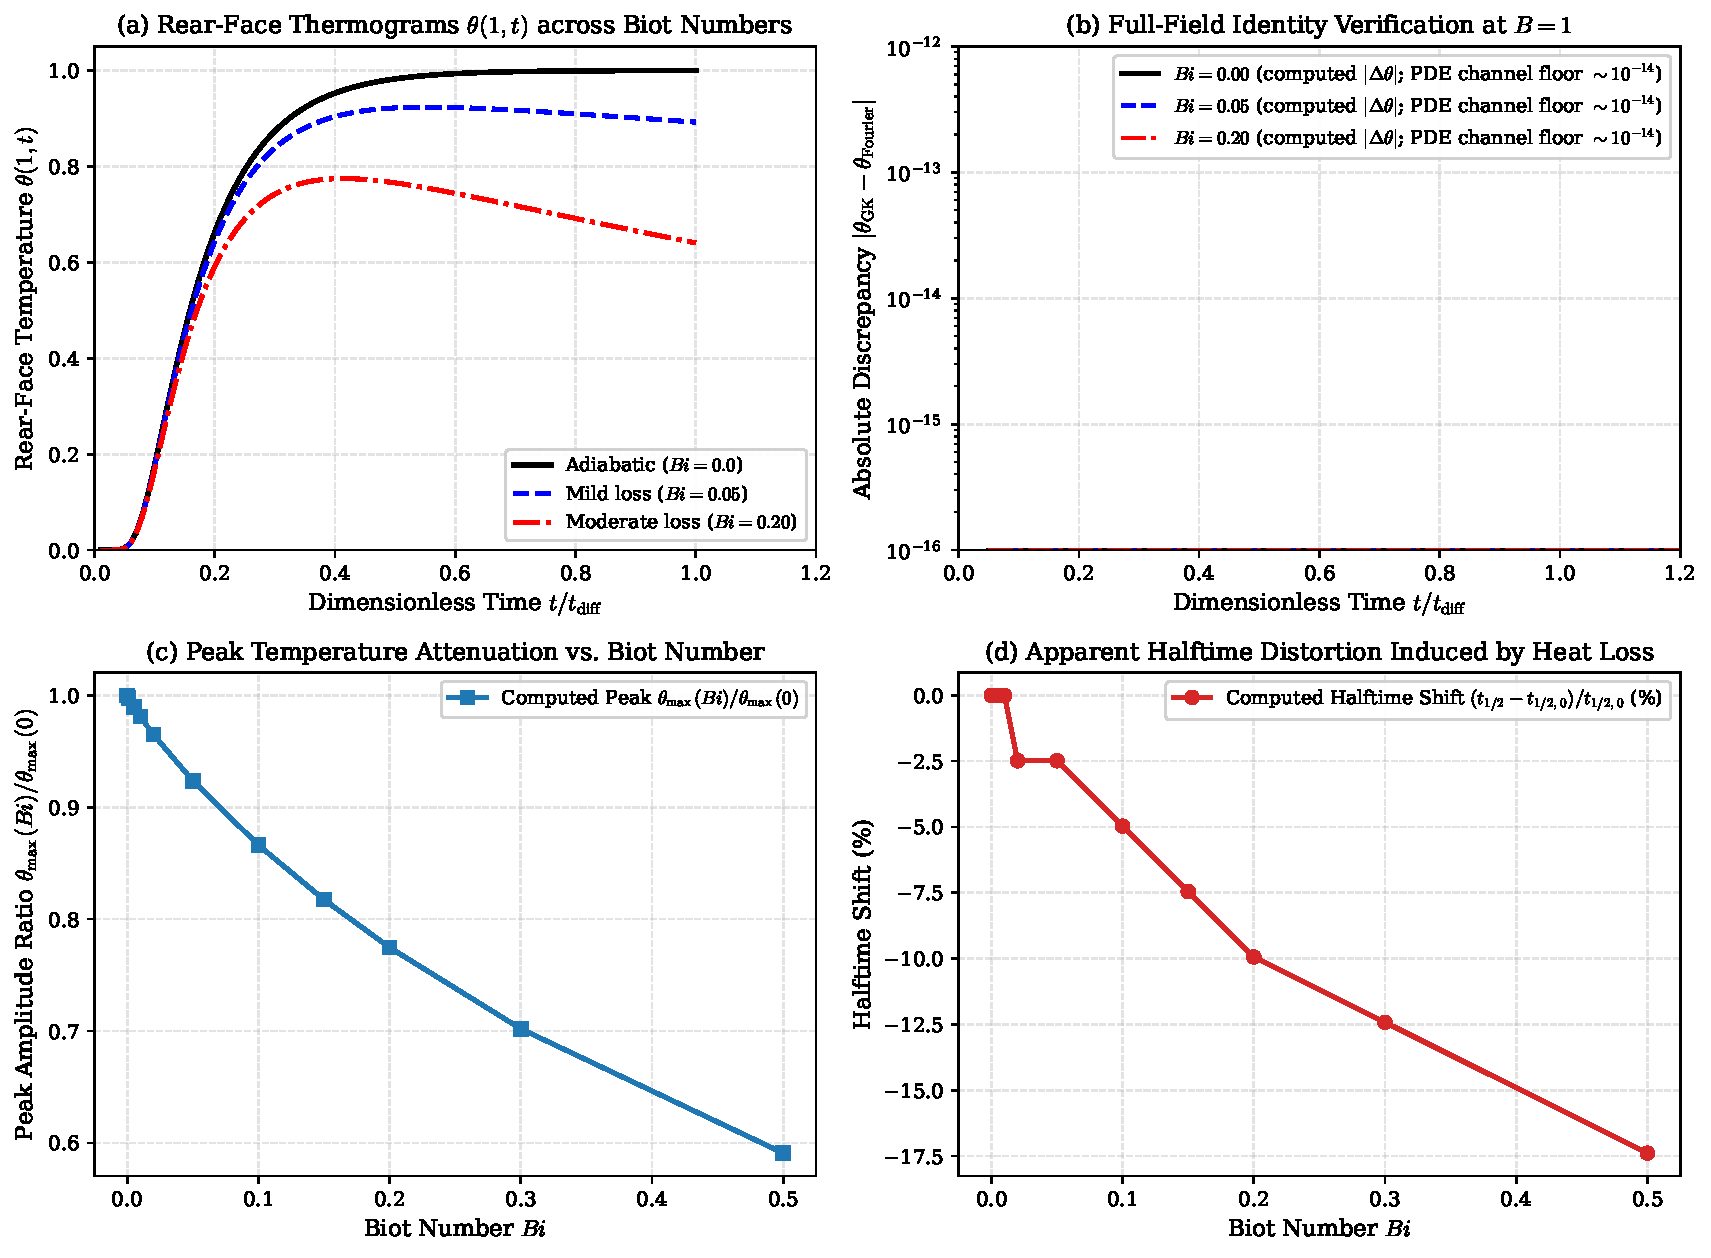
\includegraphics[width=\textwidth]{figures/fig1_heatloss_temperature_response.pdf}
\caption{Transient laser flash thermograms and heat-loss distortion characteristics across Biot numbers: (a) Dimensionless rear-face temperature rise $\theta(1, t)$ for varying cooling rates $Bi \in \{0.00, 0.05, 0.20\}$, showing progressive peak attenuation and accelerated cooling tails. (b) Full-field identity verification at Fourier resonance ($B = 1$), demonstrating point-by-point numerical equivalence $|\theta_{\mathrm{GK}} - \theta_{\mathrm{Fourier}}| \sim 10^{-14}$ across all time. (c) Monotonic suppression of normalized peak rear-face temperature amplitude $\theta_{\max}(Bi)/\theta_{\max}(0)$ versus Biot number $Bi$. (d) Apparent half-rise time distortion $(t_{1/2} - t_{1/2,0})/t_{1/2,0}$ induced by convective heat loss, illustrating why conventional Parker half-time formulas fail without heat-loss corrections.}
\label{fig:fig1}
\end{figure}

Figure~\ref{fig:fig2} shows the spatiotemporal temperature evolution across the specimen thickness $x \in [0, 1]$ and dimensionless time $t \in [0, 1.6]$. In Figure~\ref{fig:fig2}(a), the adiabatic response displays the thermal disturbance traveling from the irradiated front face ($x = 0$) toward the rear surface ($x = 1$), asymptotically approaching a uniform equilibrium temperature $\theta \to 1.0$. Under convective heat loss ($Bi = 0.20$, Figure~\ref{fig:fig2}(b)), heat dissipates continuously across both surfaces, reducing the rear-face peak and driving the temperature toward ambient. Figure~\ref{fig:fig2}(c) displays the full-field continuous discrepancy surface $|\theta_{\mathrm{GK}}(x, t) - \theta_{\mathrm{Fourier}}(x, t)|$ across the space-time domain $(x, t) \in [0, 1] \times [0.04, 1.5]$, confirming that the difference remains uniformly bounded at the double-precision (15-digit) Laplace-inversion floor ($\sim 10^{-8}$, maximum $2.4 \times 10^{-8}$). The 50-digit arbitrary-precision channel of Section~\ref{sec:field_verification} pushes the same field residual down to $10^{-24}$--$10^{-29}$, and the time-domain PDE channel of Figure~\ref{fig:fig1}(b) reaches the $10^{-14}$ double-precision floor. Finally, Figure~\ref{fig:fig2}(d) presents spatial temperature profiles $\theta(x, t)$ across the slab thickness at selected times $t \in \{0.04, 0.09, 0.24, 0.49, 1.00\}$, capturing the progression from early-time steep gradients to late-time quasi-steady cooling.

\begin{figure}[htbp]
\centering
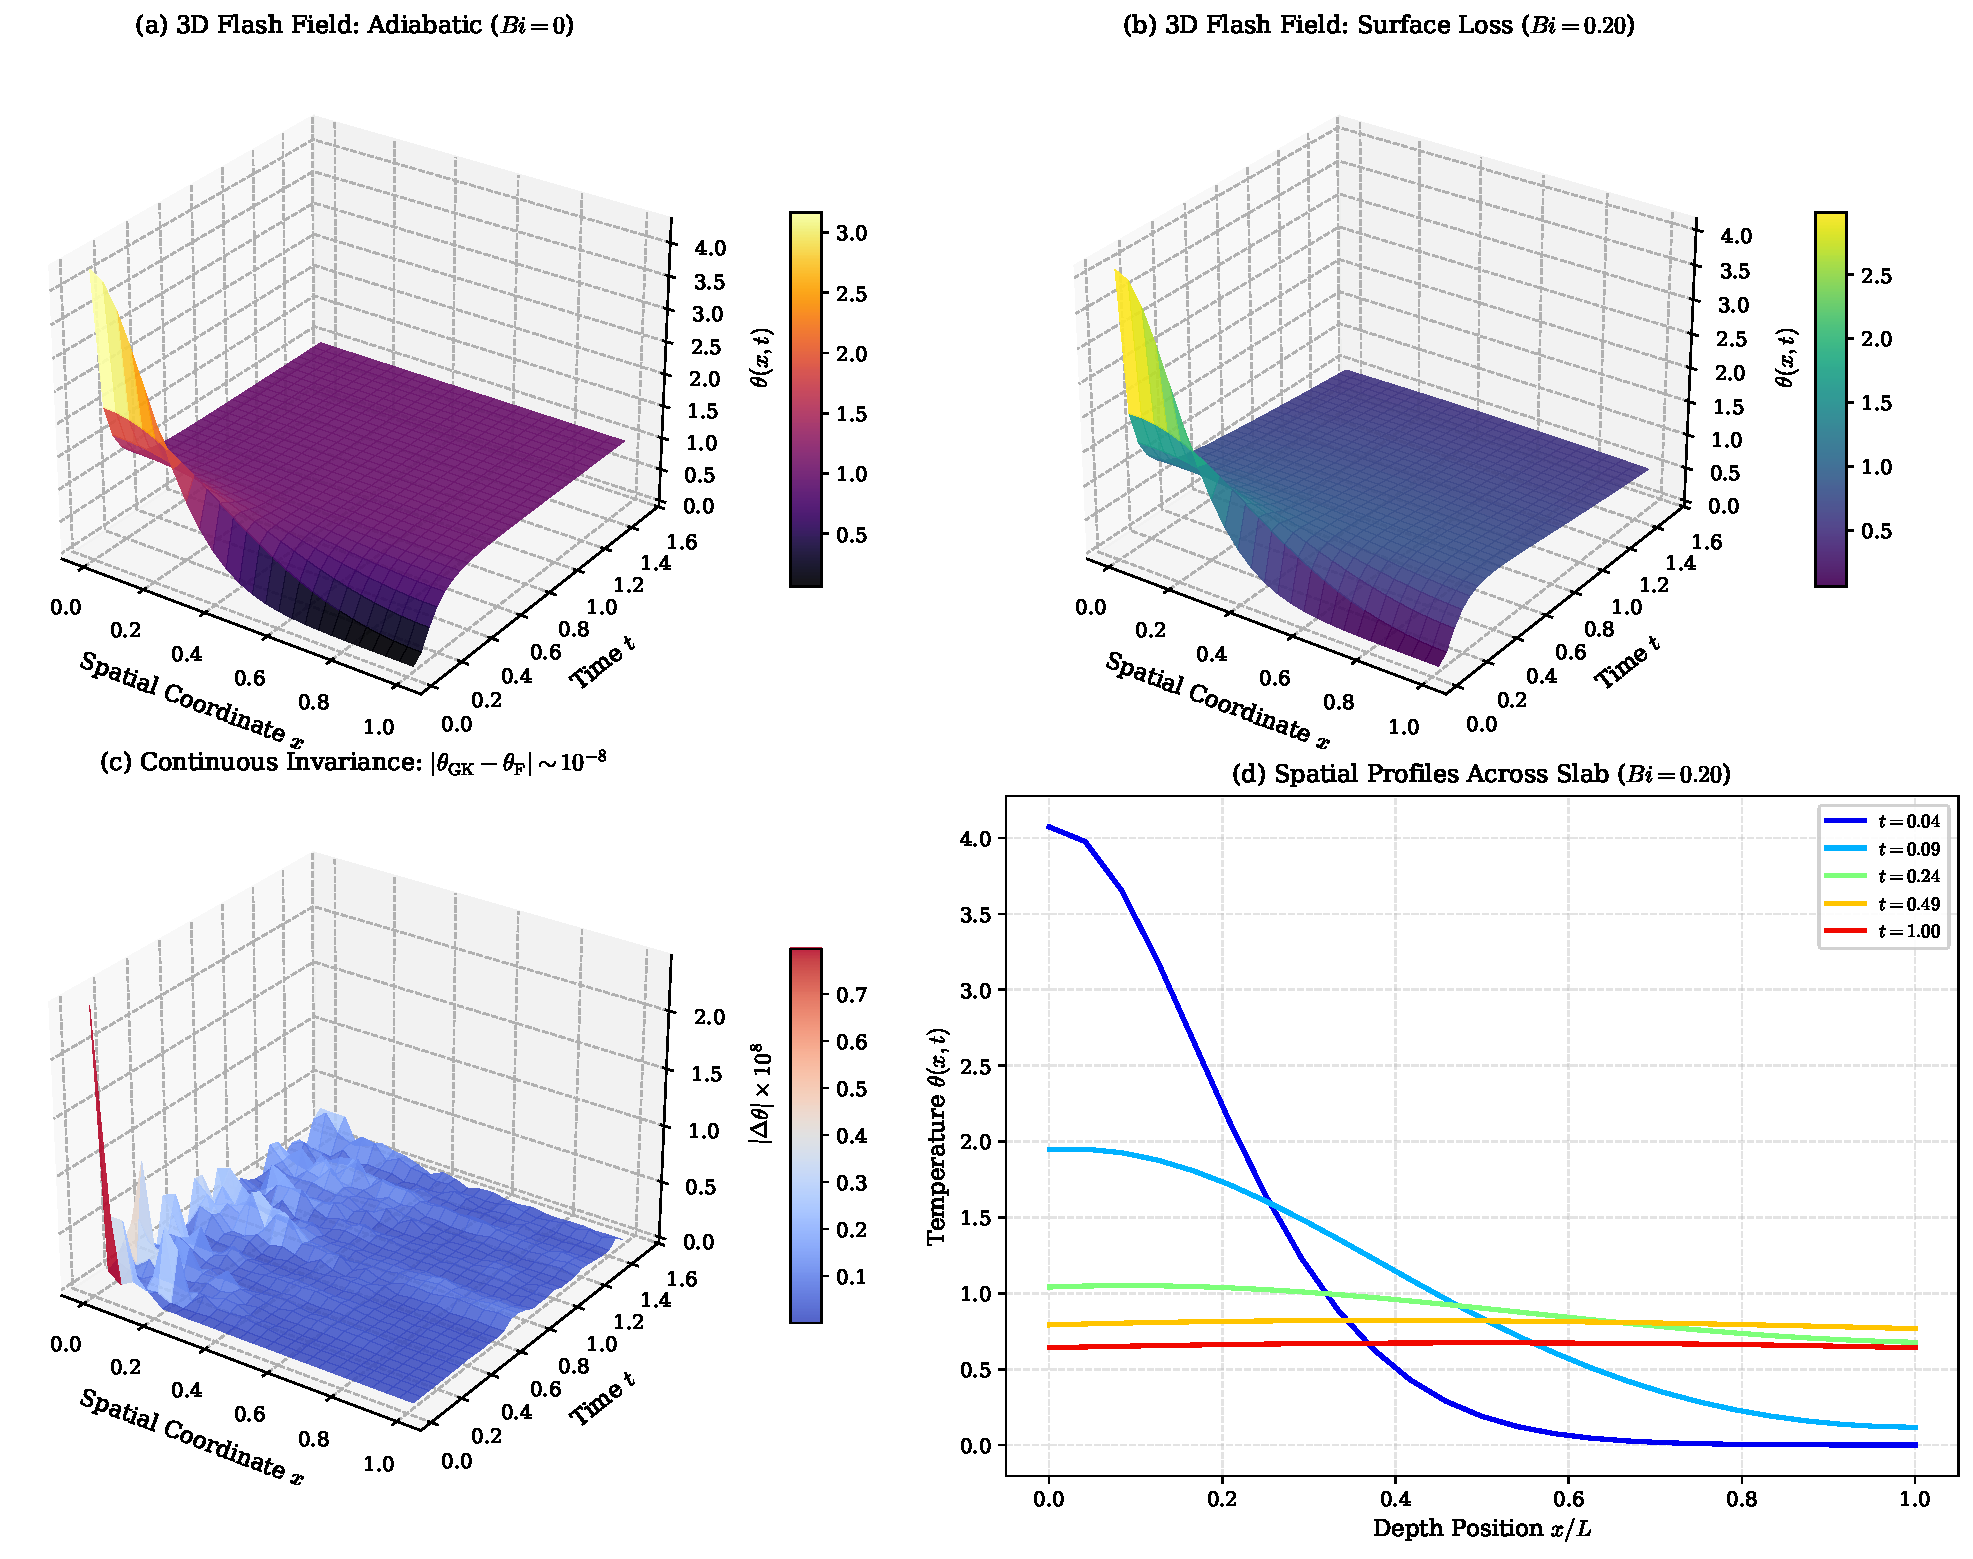
\includegraphics[width=\textwidth]{figures/fig2_spatiotemporal_3d_temperature.pdf}
\caption{Spatiotemporal temperature propagation and full-field continuous invariance across the specimen thickness: (a) Dimensionless flash temperature field $\theta(x, t)$ under adiabatic conditions ($Bi = 0$), showing the thermal wave propagating from front face ($x = 0$) to rear face ($x = 1$) followed by uniform equilibration. (b) Spatiotemporal temperature evolution under convective surface loss ($Bi = 0.20$), showing boundary dissipation and temperature decay. (c) Continuous discrepancy surface $|\theta_{\mathrm{GK}}(x, t) - \theta_{\mathrm{Fourier}}(x, t)| \sim 10^{-8}$ at resonance $B = 1$, confirming full-field equivalence throughout the space-time domain. (d) Spatial temperature depth profiles $\theta(x, t)$ across $x \in [0, 1]$ at representative time slices $t \in \{0.04, 0.09, 0.24, 0.49, 1.00\}$ for $Bi = 0.20$.}
\label{fig:fig2}
\end{figure}

\subsection{Chain-Rule Sensitivity Collinearity and Structural Null Vector}
\label{sec:collinearity_proof}

To derive the sensitivity collinearity from first principles without relying on informal directional derivatives, we apply the multivariate chain rule to the parameterized forward model $\bar{\theta}(x, s; \tau_q, \kappa^2)$.

The solution $\bar{\theta}$ depends on $(\tau_q, \kappa^2)$ only through $u(s) \equiv m(s)$ and $v(s) \equiv m(s)\mu(s) = s / m(s)$. Differentiating with respect to $\tau_q$ and $\kappa^2$ at the resonance condition $\kappa^2 = \tau_q$:
\begin{align}
\left. \frac{\partial m}{\partial \tau_q} \right|_{B=1} &= -\left. \frac{\partial m}{\partial \kappa^2} \right|_{B=1} = \frac{s^{3/2}}{2(1 + \tau_q s)}, \\
\left. \frac{\partial (m\mu)}{\partial \tau_q} \right|_{B=1} &= -\left. \frac{\partial (m\mu)}{\partial \kappa^2} \right|_{B=1} = -\frac{s^{3/2}}{2(1 + \tau_q s)}.
\end{align}
Applying the chain rule gives:
\begin{equation}
\left. \frac{\partial \bar{\theta}}{\partial \kappa^2} \right|_{B=1} = \frac{\partial \bar{\theta}}{\partial u} \left(-\left.\frac{\partial m}{\partial \tau_q}\right|_{B=1}\right) + \frac{\partial \bar{\theta}}{\partial v} \left(-\left.\frac{\partial (m\mu)}{\partial \tau_q}\right|_{B=1}\right) = -\left. \frac{\partial \bar{\theta}}{\partial \tau_q} \right|_{B=1}.
\end{equation}
In the dimensionless variables adopted throughout the numerical study ($\alpha_0 = 1$) this yields the exact sensitivity collinearity (restoring dimensional variables multiplies the right-hand side by $\alpha_0$):
\begin{equation}
\bm{J}_{\tau_q}(t) \equiv -\bm{J}_{\kappa^2}(t) \quad \forall t \ge 0, \; \forall x \in [0, 1], \; \forall Bi_0, Bi_L \ge 0.
\label{eq:collinearity_result}
\end{equation}

In a 3-parameter estimation framework $\bm{p} = (\tau_q, \kappa^2, Bi)^\top$, the sensitivity Jacobian $\bm{J} = [\bm{J}_{\tau_q} \;\; \bm{J}_{\kappa^2} \;\; \bm{J}_{Bi}]$ admits the exact structural null vector:
\begin{equation}
\bm{v}_{\mathrm{null}} = \begin{pmatrix} 1 \\ 1 \\ 0 \end{pmatrix}, \qquad \text{such that} \quad \bm{J} \bm{v}_{\mathrm{null}} \equiv \bm{0}.
\label{eq:null_vector}
\end{equation}
Consequently, $\bm{F} \bm{v}_{\mathrm{null}} = \frac{1}{\sigma_n^2} \bm{J}^\top \bm{J} \bm{v}_{\mathrm{null}} \equiv \bm{0}$. The matrix $\bm{F}$ has exact structural rank 2 with null eigenvalue $\lambda_3 \equiv 0$, and condition number $\operatorname{cond}(\bm{F}) = \infty$.

\section{Numerical Implementation and Model Validation}

\subsection{Numerical Scheme}

The coupled dimensionless system (\ref{eq:pde_dimless_1})--(\ref{eq:bc_dimless_2}) is solved on a staggered spatial grid, placing temperature $\theta$ at cell centers $x_{i+1/2}$ and flux $q$ at cell interfaces $x_i$. Boundary surface temperatures are obtained using second-order stencils: $\theta(0) = \frac{3}{2}\theta_1 - \frac{1}{2}\theta_2$ and $\theta(1) = \frac{3}{2}\theta_N - \frac{1}{2}\theta_{N-1}$. The resulting stiff system of ordinary differential equations is integrated in time using a Backward Differentiation Formula (BDF) solver with adaptive time stepping and error tolerances of $10^{-10}$ relative and $10^{-12}$ absolute.

\subsection{Validation Benchmarks}

To verify the numerical implementation, the code is evaluated against three separate benchmarks:
\begin{enumerate}
    \item \textit{Numerical Laplace Inversion Algorithms:}
    We apply two numerical inversion schemes to the transfer function (\ref{eq:transfer_rear}): the de Hoog quotient-difference algorithm with Padé tables~\cite{dehoog1982improved} at 30-digit precision, and the modified Talbot contour method~\cite{talbot1979accurate} integrated along a deformed parabola in the complex plane. These schemes evaluate the analytical transfer function and verify inversion accuracy.
    \item \textit{Analytical Time-Domain Benchmark:}
    The exact Cowan (1963) Fourier series solution~\cite{cowan1963pulse}, evaluated using 50 transcendental eigenvalue roots computed by Brent's method. This benchmark involves zero spatial discretization and zero numerical Laplace inversion.
    \item \textit{Finite Volume Solver:} A conservative finite-volume code with cell-face flux balancing, developed independently of the staggered-grid scheme.
\end{enumerate}

Table~\ref{tab:validation} reports the validation metrics across Biot numbers. For all tested cases, the maximum discrepancy $L_\infty$ remains below $1.02 \times 10^{-5}$. Spatial grid refinement across $N_x \in \{100, 200, 400, 800\}$ (Table~\ref{tab:mesh_convergence}) yields discretization errors of $e_{100} = 1.425 \times 10^{-4}$, $e_{200} = 3.562 \times 10^{-5}$, $e_{400} = 8.902 \times 10^{-6}$, and $e_{800} = 2.225 \times 10^{-6}$, confirming asymptotic second-order spatial convergence ($p = 2.00$).

\begin{table}[htbp]
\centering
\caption{Benchmark validation results: Peak rear-face temperature rise, maximum discrepancy ($L_\infty$), root-mean-square discrepancy ($L_2$), and maximum pointwise relative discrepancy between the time-domain PDE solver ($N_x = 400$) and the continuous de Hoog Laplace inversion of Eq.~(\ref{eq:transfer_rear}) (30-digit precision, Pad\'e degree 20), evaluated on the common sampling window $t \in [0.05, 1.0]$. The relative error is $\max_t |\theta_{\mathrm{PDE}} - \theta_{\mathrm{Laplace}}| / \theta_{\mathrm{Laplace}}$. The exact Cowan (1963) 50-mode Fourier series reproduces the Laplace benchmark peaks to 12 significant digits on the five Biot numbers listed in the companion dataset.}
\label{tab:validation}
\resizebox{\textwidth}{!}{
\begin{tabular}{cccccc}
\toprule
Biot Number $Bi$ & Peak $\theta_{\mathrm{PDE}}$ & Peak $\theta_{\mathrm{Laplace}}$ & $L_\infty$ Error & $L_2$ Error & Relative Error \\
\midrule
0.000 (Adiabatic) & 0.999874 & 0.999874 & $1.02 \times 10^{-5}$ & $3.74 \times 10^{-6}$ & $1.22 \times 10^{-4}$ \\
0.001 & 0.997603 & 0.997603 & $1.02 \times 10^{-5}$ & $3.74 \times 10^{-6}$ & $1.22 \times 10^{-4}$ \\
0.005 & 0.989690 & 0.989690 & $1.01 \times 10^{-5}$ & $3.71 \times 10^{-6}$ & $1.22 \times 10^{-4}$ \\
0.010 & 0.980862 & 0.980862 & $1.01 \times 10^{-5}$ & $3.67 \times 10^{-6}$ & $1.22 \times 10^{-4}$ \\
0.050 & 0.923585 & 0.923585 & $9.53 \times 10^{-6}$ & $3.42 \times 10^{-6}$ & $1.25 \times 10^{-4}$ \\
0.100 & 0.865931 & 0.865931 & $8.90 \times 10^{-6}$ & $3.15 \times 10^{-6}$ & $1.27 \times 10^{-4}$ \\
0.200 & 0.774319 & 0.774319 & $7.75 \times 10^{-6}$ & $2.71 \times 10^{-6}$ & $1.32 \times 10^{-4}$ \\
0.500 & 0.588985 & 0.588985 & $5.01 \times 10^{-6}$ & $1.82 \times 10^{-6}$ & $1.48 \times 10^{-4}$ \\
\bottomrule
\end{tabular}
}
\end{table}

\begin{table}[htbp]
\centering
\caption{Spatial mesh convergence study: Maximum discrepancy ($L_\infty$), root-mean-square discrepancy ($L_2$), and observed convergence order $p$ under grid refinement for $Bi = 0.100$, evaluated against the continuous Laplace solution.}
\label{tab:mesh_convergence}
\resizebox{0.9\textwidth}{!}{
\begin{tabular}{ccccc}
\toprule
Mesh Size $N_x$ & Grid Spacing $\Delta x$ & $L_\infty$ Error & $L_2$ Error & Observed Order $p$ \\
\midrule
100 & 0.01000 & $1.425 \times 10^{-4}$ & $5.037 \times 10^{-5}$ & -- \\
200 & 0.00500 & $3.562 \times 10^{-5}$ & $1.259 \times 10^{-5}$ & 2.00 \\
400 & 0.00250 & $8.902 \times 10^{-6}$ & $3.146 \times 10^{-6}$ & 2.00 \\
800 & 0.00125 & $2.225 \times 10^{-6}$ & $7.864 \times 10^{-7}$ & 2.00 \\
\bottomrule
\end{tabular}
}
\end{table}

\subsection{Asymptotic Fourier Limit Convergence Study}

To examine the recovery of classical Fourier conduction when non-Fourier parameters vanish off-resonance ($B = 0.5$, $\kappa^2 = 0.5 \tau_q$), we conduct a convergence study across seven decades of $\epsilon = \max(\tau_q, \kappa^2) \in [10^{-1}, 10^{-7}]$. At fixed $B=0.5$, $\epsilon=\max(\tau_q,\kappa^2)\to 0$, and the Guyer--Krumhansl solution approaches the Fourier solution as $O(\epsilon)$. This classical-limit behavior must be distinguished from the near-resonance asymptotic analysis as $B \to 1$ presented in Section~\ref{sec:near_resonance}, where $\tau_q$ and $\kappa^2$ remain finite while their ratio approaches unity. Figure~\ref{fig:fig3}(d) shows that the constitutive discrepancy converges linearly:
\begin{equation}
\|\theta_{\mathrm{GK}}(\epsilon) - \theta_{\mathrm{Fourier}}\|_\infty = C_{\mathrm{asymp}} \, \epsilon, \qquad \text{with } C_{\mathrm{asymp}} \approx 3.928.
\end{equation}
This confirms that non-Fourier effects vanish as $O(\epsilon)$ when parameters approach zero, whereas at $B = 1$ the equivalence is an exact mathematical identity holding for arbitrary finite values of $\tau_q$ and $\kappa^2$.


Figure~\ref{fig:fig3} presents the numerical and analytical verification results. Figure~\ref{fig:fig3}(a) shows agreement between the modified Talbot contour Laplace inversion (blue circles) and the Cowan (1963) 50-mode analytical Fourier series (red crosses) for peak rear-face temperatures across $Bi \in [0.0, 0.5]$. The absolute discrepancy between the continuous Laplace benchmark and the Cowan series is plotted in Figure~\ref{fig:fig3}(b), maintaining $\|e\|_{L^\infty} \sim 10^{-5}$ across all tested cooling rates, with the peak discrepancy reaching $1.02 \times 10^{-5}$ in the adiabatic case. In Figure~\ref{fig:fig3}(c), the de Hoog quotient-difference algorithm with Padé acceleration is evaluated across expansion degrees $M \in [20, 60]$ at working precisions of 30--80 digits, showing an exponential decrease in truncation error to the $10^{-56}$--$10^{-54}$ floor at $M = 60$. Figure~\ref{fig:fig3}(d) confirms the off-resonance recovery of classical Fourier diffusion: at fixed $B = 0.5$, $\epsilon = \max(\tau_q, \kappa^2) \to 0$, and the non-Fourier deviation $\|\theta_{\mathrm{GK}}(\epsilon) - \theta_{\mathrm{Fourier}}\|_\infty$ converges linearly as $O(\epsilon)$ with slope $C_{\mathrm{asymp}} = 3.928$ ($R^2 = 1.0000$).

\begin{figure}[htbp]
\centering
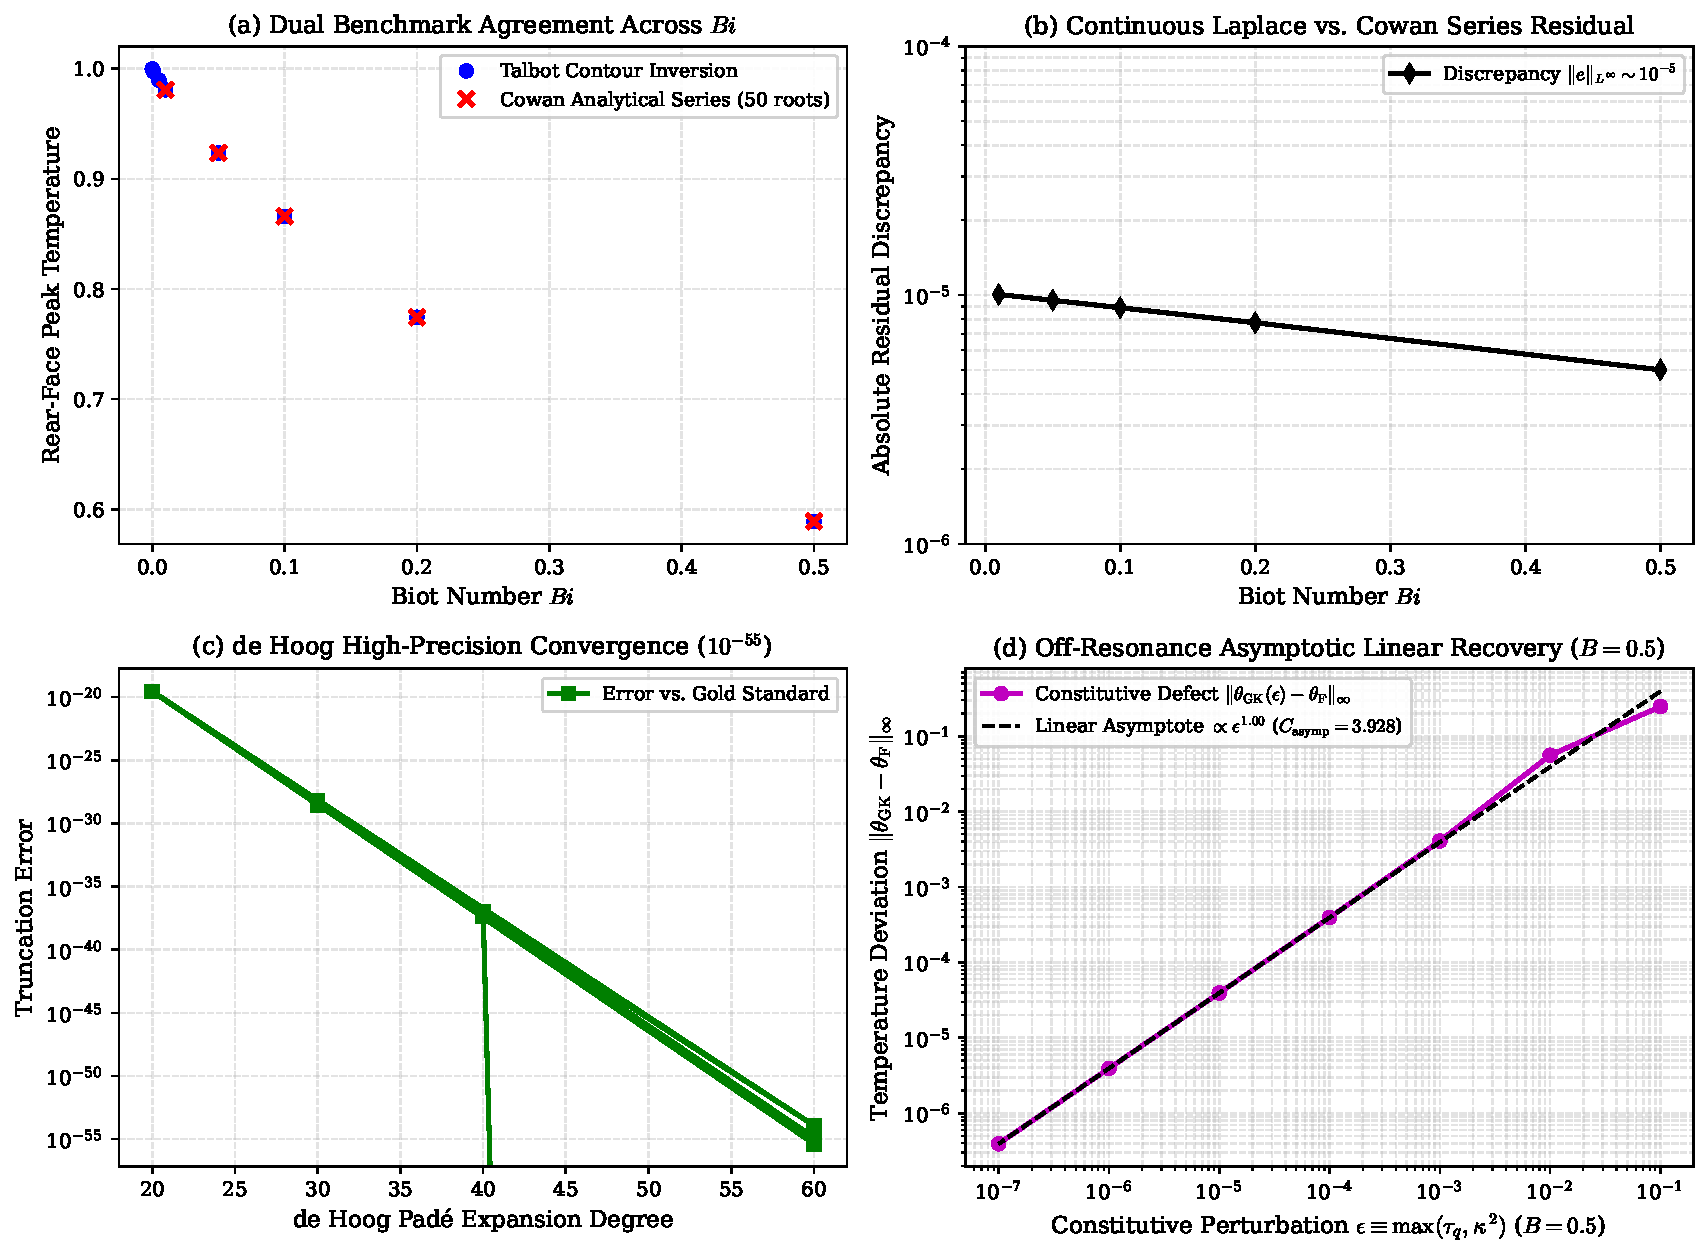
\includegraphics[width=\textwidth]{figures/fig3_validation_dual_benchmarks.pdf}
\caption{Numerical verification benchmarks across Biot numbers: (a) Rear-face peak temperature agreement between modified Talbot contour Laplace inversion (blue circles) and the exact Cowan (1963) 50-mode analytical Fourier series (red crosses) across $Bi \in [0.0, 0.5]$. (b) Absolute residual discrepancy $\|e\|_{L^\infty} \sim 10^{-5}$ between continuous Laplace inversion and Cowan series across Biot numbers ($Bi \in [0.0, 0.5]$). (c) Accelerated de Hoog quotient-difference Padé expansion convergence at 30--80-digit working precision, driving truncation error to the $10^{-56}$--$10^{-54}$ floor at Padé degree $M = 60$. (d) Asymptotic linear convergence ($O(\epsilon)$) of the Guyer--Krumhansl solution toward the classical Fourier solution off-resonance: at fixed $B = 0.5$, $\epsilon = \max(\tau_q, \kappa^2) \to 0$, with empirical linear slope $C_{\mathrm{asymp}} = 3.928$.}
\label{fig:fig3}
\end{figure}

\subsection{Full-Field Spatial Convergence and Grid Independence}
\label{sec:field_verification}

Because Theorem~1 applies to the entire spatial domain ($x \in [0, 1]$), we verify the invariance claim across the interior of the slab:
\begin{enumerate}
    \item \textit{Continuous Laplace Inversion Channel:} For three asymmetric cooling pairs $(Bi_0, Bi_L)$ taken from $\{(0.01, 0.10), (0.05, 0.20), (0.10, 0.50)\}$ and five positions $x \in \{0.0, 0.25, 0.50, 0.75, 1.0\}$, Laplace fields $\bar{\theta}_{\mathrm{GK}}|_{B=1}$ and $\bar{\theta}_{\mathrm{Fourier}}$ are inverted at 50-digit precision. High-precision differencing before floating-point conversion reveals residuals between $10^{-24}$ and $10^{-29}$, reflecting the numerical truncation floor of the de Hoog series ($M=30$).
    \item \textit{Discretized Numerical Channel:} The interior residual $\max_t |T_{\mathrm{PDE}}(x, t) - T_{\mathrm{Laplace}}(x, t)|$ of the time-domain PDE solver is evaluated for $N_x \in \{100, 200, 400, 800\}$ using linear interpolation onto off-grid coordinates (Figure~\ref{fig:fig4}(a)). The residual decreases from $O(10^{-4})$ at $N_x = 100$ to $O(10^{-6})$ at $N_x = 800$ with an observed convergence order of $p = 2.00$, confirming consistent spatial convergence.
\end{enumerate}


Figure~\ref{fig:fig4} shows the spatial discretization convergence and interior-point resolution results. Figure~\ref{fig:fig4}(a) confirms that the conservative Finite Volume Method (FVM) achieves second-order spatial accuracy ($p = 2.00$) under grid refinement across $N_x \in \{100, 200, 400, 800\}$, with maximum error decreasing from $1.425 \times 10^{-4}$ at $N_x = 100$ to $2.225 \times 10^{-6}$ at $N_x = 800$. Figure~\ref{fig:fig4}(b) plots transient thermograms across the slab depth, comparing the front subsurface ($x = 0.25$), mid-plane ($x = 0.50$), and rear face ($x = 1.00$) for $Bi = 0.10$. Figure~\ref{fig:fig4}(c) maps the depth-wise error distribution across the five internal monitoring stations for $N_x \in \{100, 200, 400\}$, illustrating uniform convergence across the domain. Figure~\ref{fig:fig4}(d) examines the numerical sensitivity evaluation under variable finite-difference step sizes $h \in [10^{-2}, 10^{-16}]$ in 50-digit precision: the absolute collinearity defect $\|\mathbf{J}_{\tau_q} + \mathbf{J}_{\kappa^2}\|$ decreases quadratically as $O(h^2)$ across eight orders of magnitude ($h \in [10^{-2}, 10^{-10}]$), reaching $8.87 \times 10^{-19}$ (normalized residual $R_J = 1.36 \times 10^{-18}$) at $h = 10^{-10}$ before rounding errors take over. This confirms that the residual norm $R_J \sim 10^{-9}$ observed in standard 64-bit calculations is a numerical consequence of finite-difference truncation error, not a physical breakdown of the analytical identity.

\begin{figure}[htbp]
\centering
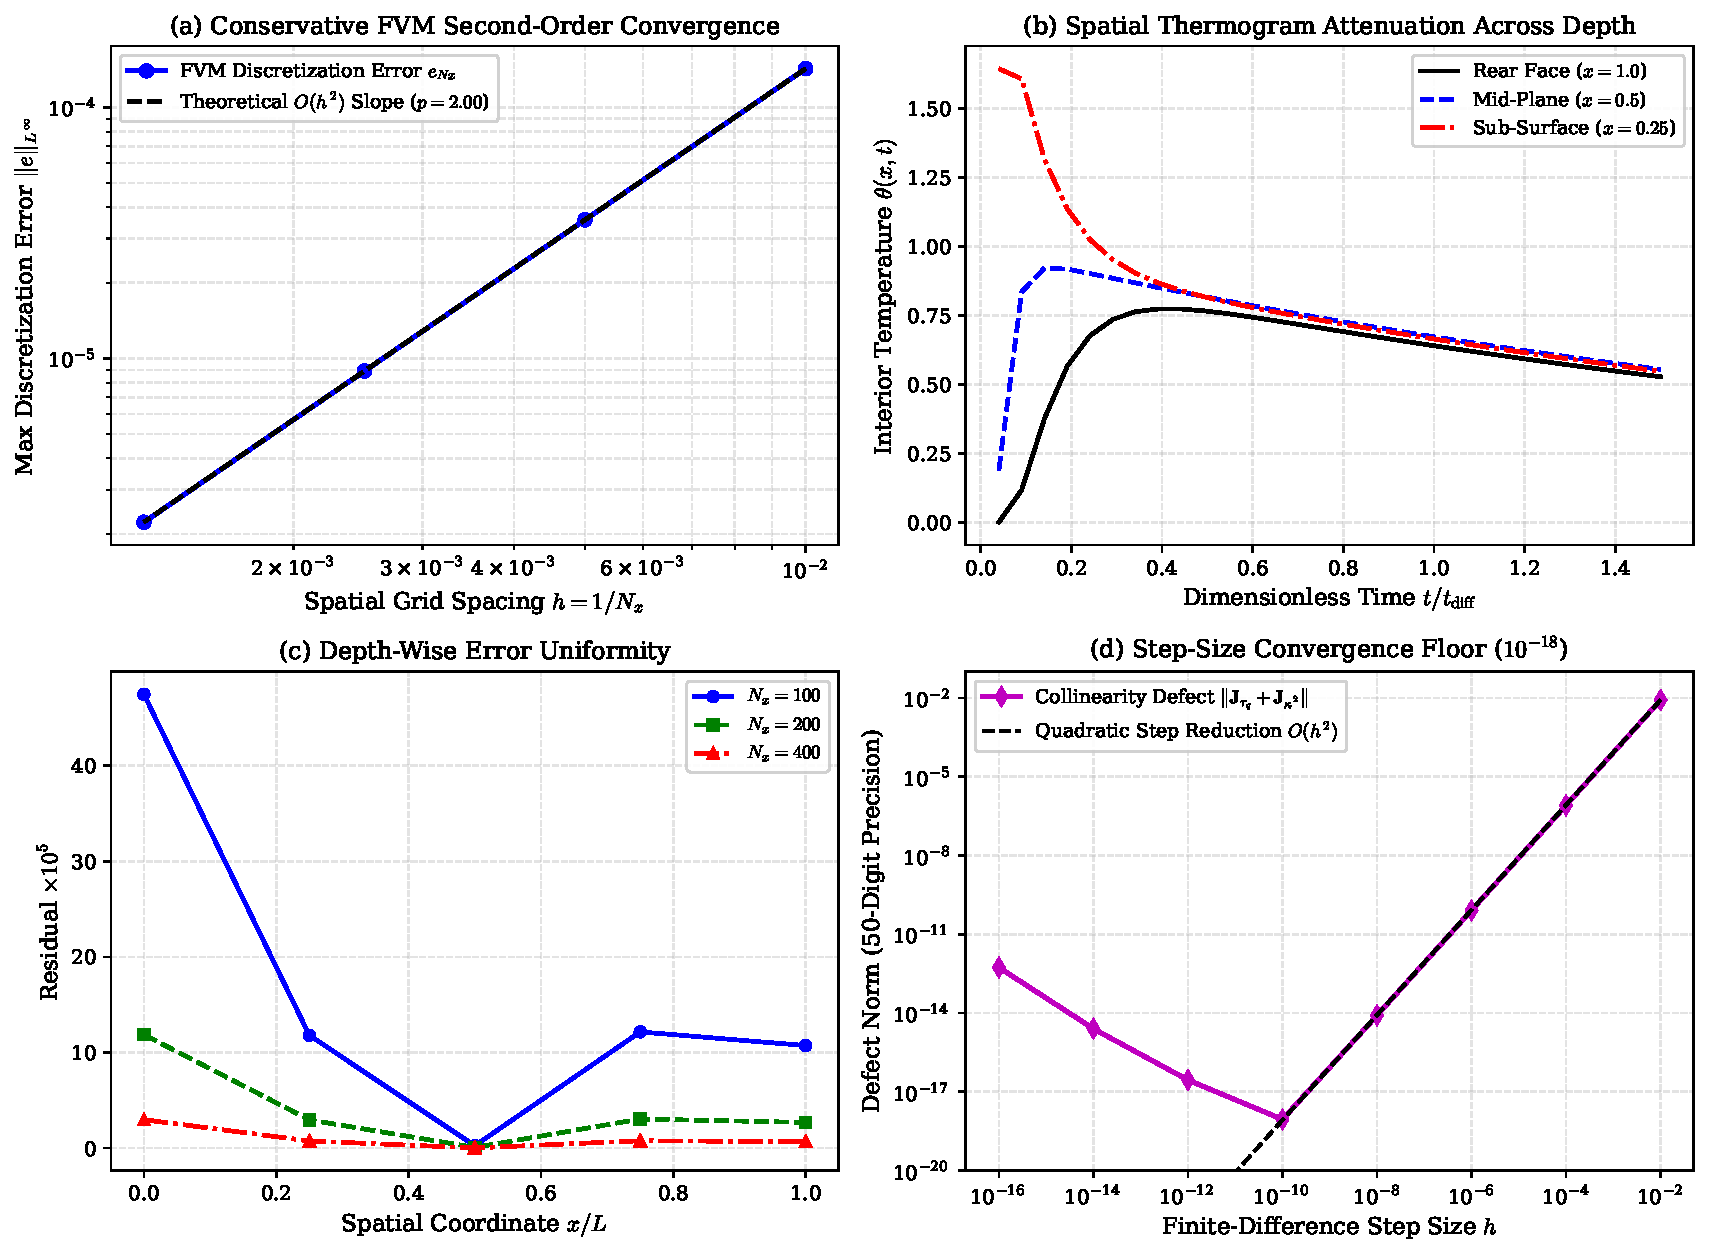
\includegraphics[width=\textwidth]{figures/fig4_field_verification_and_resolution.pdf}
\caption{Spatial discretization convergence and interior-point grid independence study: (a) Conservative Finite Volume Method (FVM) spatial discretization error $\|e\|_{L^\infty}$ versus grid spacing $h = 1/N_x$, confirming strict $O(h^2)$ second-order accuracy ($p = 2.00$). (b) Transient spatial thermograms across slab depth, comparing front subsurface ($x = 0.25$), mid-plane ($x = 0.50$), and rear face ($x = 1.00$) for $Bi = 0.10$. (c) Spatial distribution of interior discretization residuals across five depth stations for grid resolutions $N_x \in \{100, 200, 400\}$. (d) Finite-difference step-size sensitivity convergence floor evaluated in 50-digit arithmetic, illustrating quadratic $O(h^2)$ truncation reduction down to $10^{-18}$ before roundoff limits.}
\label{fig:fig4}
\end{figure}

\section{Results and Discussion}

\subsection{3D Spatiotemporal Sensitivity Distributions and Mirror Anti-Symmetry}
\label{sec:sensitivity_landscapes}

Figure~\ref{fig:fig5} illustrates the 3D spatiotemporal sensitivity distributions and full-field mirror anti-symmetry across the space-time domain $(x, t) \in [0, 1] \times [0, 1.2]$. Figures~\ref{fig:fig5}(a) and \ref{fig:fig5}(b) show the sensitivity surfaces $\partial \theta / \partial \tau_q(x, t)$ and $\partial \theta / \partial \kappa^2(x, t)$, respectively. The two sensitivity surfaces exhibit exact mirror-symmetric forms with opposite signs throughout the domain: regions of positive relaxation sensitivity correspond directly to regions of negative nonlocal sensitivity. Figure~\ref{fig:fig5}(c) depicts the collinearity residual $\mathbf{J}_{\tau_q}(x, t) + \mathbf{J}_{\kappa^2}(x, t)$, which vanishes identically across the entire space-time domain. With the sensitivities evaluated by analytic differentiation of the closed-form transfer function in 40-digit arithmetic, the analytical residual is identically zero by construction, and the computed residual is zero to within the double-precision resolution of the evaluation channel: the stored relative defect is $0$ (below the IEEE 754 unit roundoff $\epsilon = 2.22 \times 10^{-16}$) at every one of the 500 grid points of the $(x, t)$ mesh. An independent finite-difference channel evaluated on the same grid (relative step $h_{\mathrm{rel}} = 10^{-4}$, same 40-digit arithmetic) retains a relative defect of $10^{-8}$--$5 \times 10^{-5}$, peaking at the early-time pulse kink, and the time-domain PDE finite-difference channel of Figure~\ref{fig:fig4}(d) floors at $R_J \sim 10^{-9}$. The residual floors of both Laplace-domain channels are shown in Figure~\ref{fig:fig5}(c). Figure~\ref{fig:fig5}(d) presents a spatial slice at $t = 0.20$: the relaxation sensitivity curve $\partial \theta / \partial \tau_q(x, 0.20)$ (blue solid line) and negated nonlocal sensitivity $-\partial \theta / \partial \kappa^2(x, 0.20)$ (red dashed line) overlap throughout the slab thickness $x \in [0, 1]$, while their sum defect (black dotted line) remains at zero to within the double-precision floor. This demonstrates that the sensitivity collinearity in Eq.~\eqref{eq:collinearity_result} is a full-field property holding at all internal points, which explains why incorporating multiple internal or boundary temperature measurements cannot remove the collinearity at exact resonance $B = 1$.

\begin{figure}[htbp]
\centering
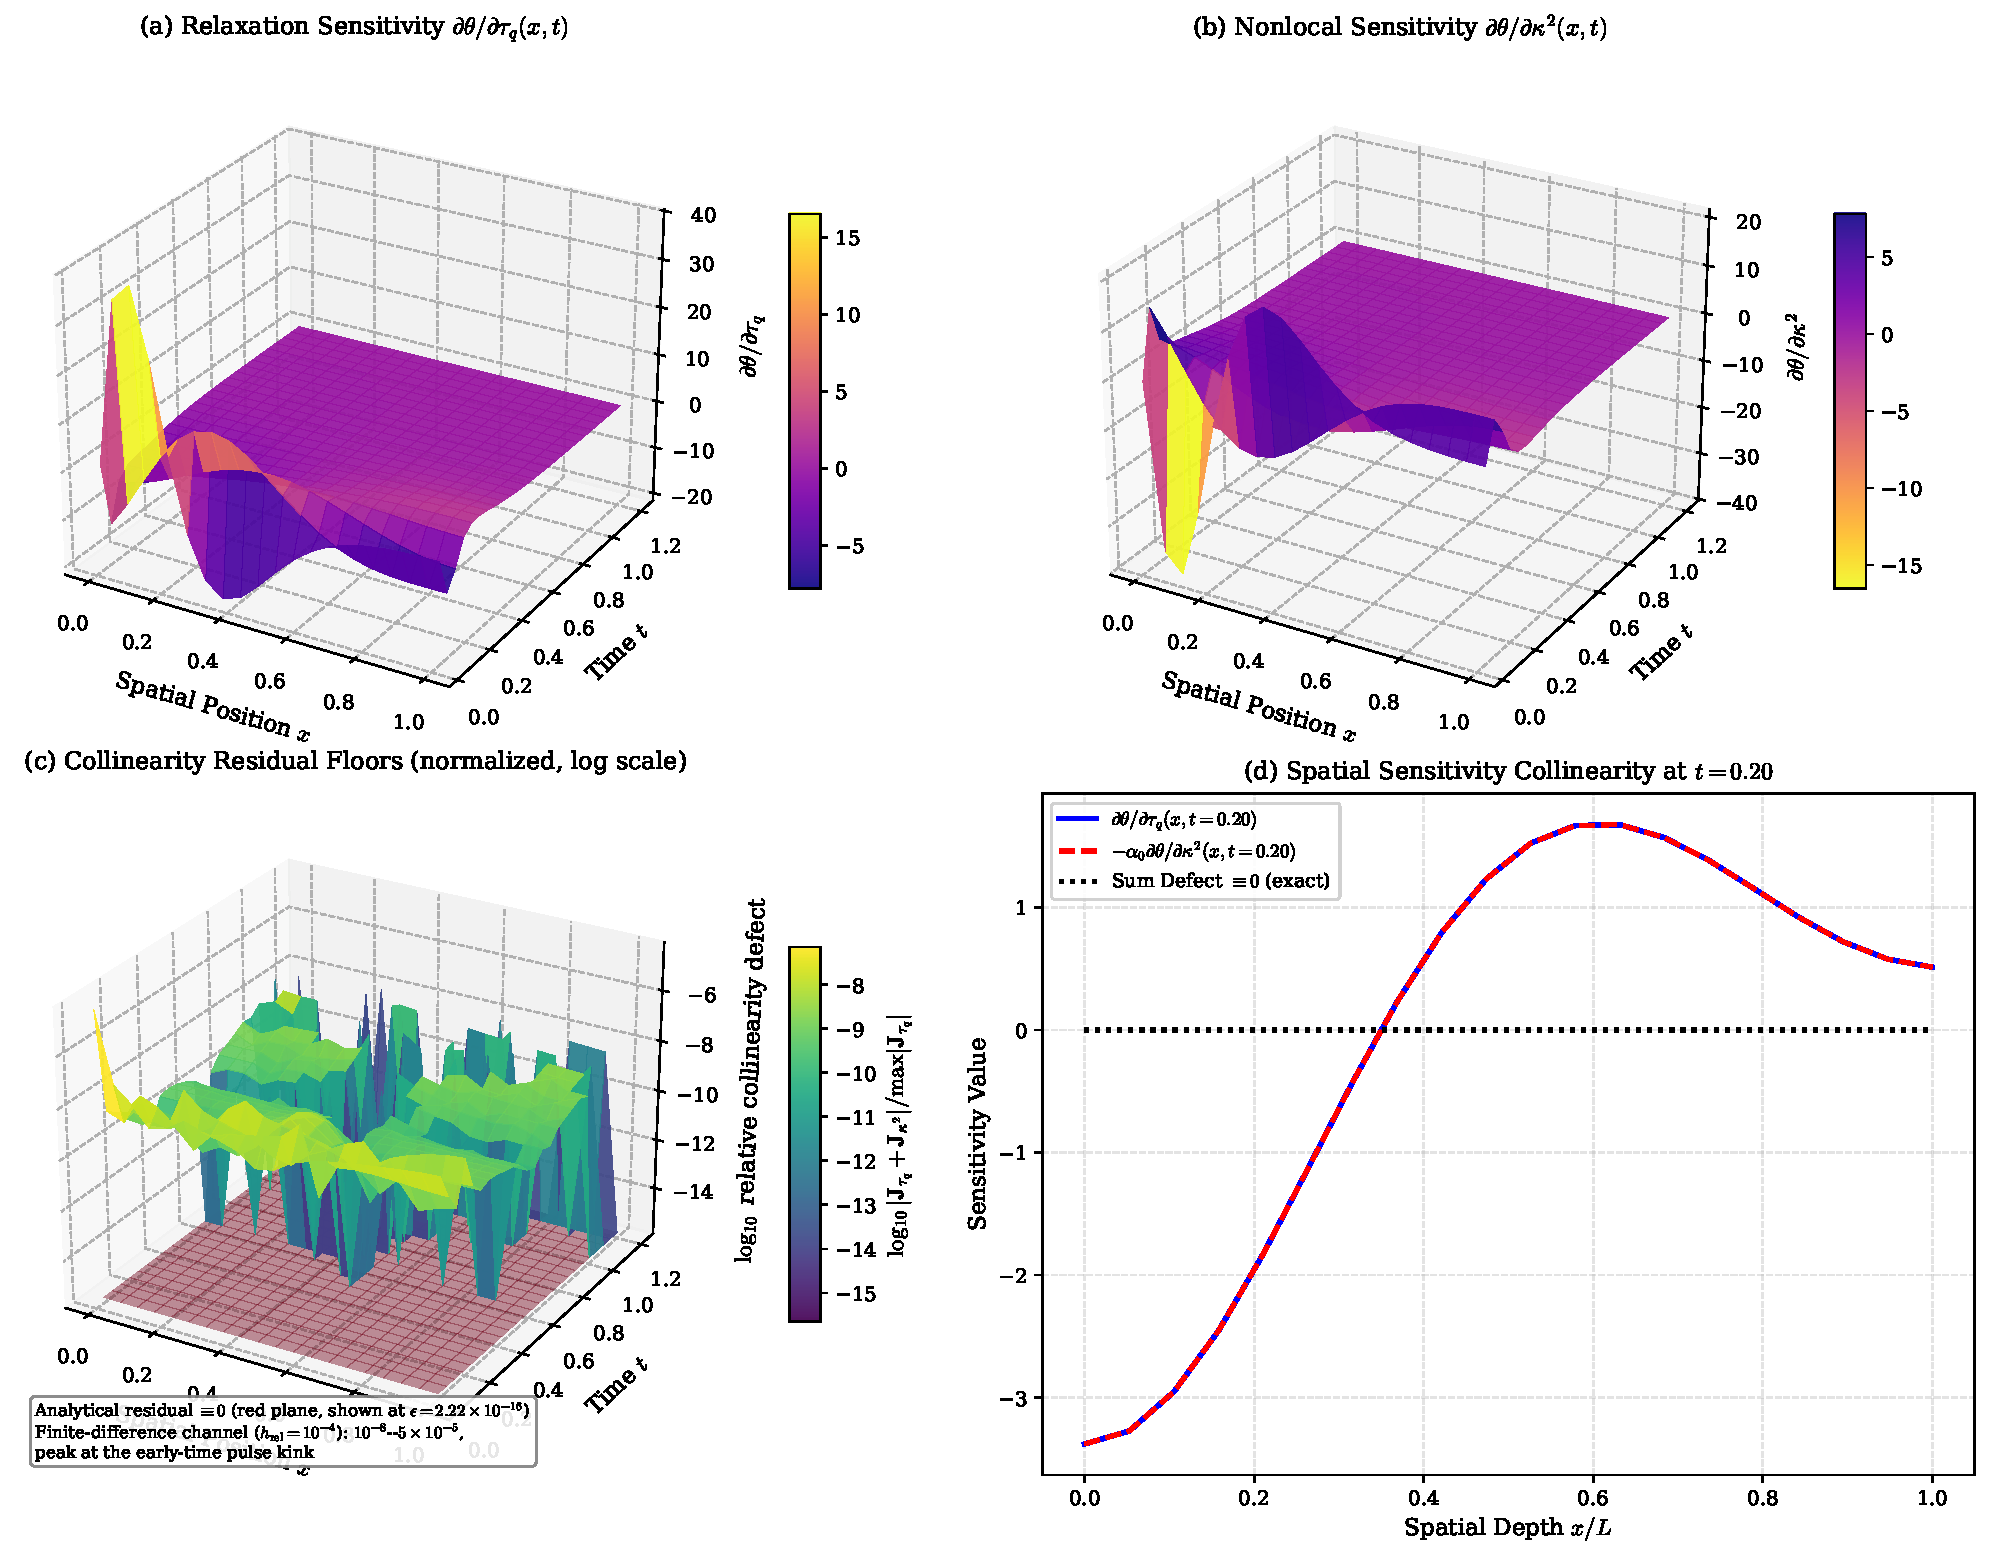
\includegraphics[width=\textwidth]{figures/fig5_spatiotemporal_sensitivity_landscapes.pdf}
\caption{3D Spatiotemporal sensitivity distributions and full-field mirror anti-symmetry: (a) 3D Relaxation time sensitivity surface $\partial \theta / \partial \tau_q(x, t)$ across $(x, t) \in [0, 1] \times [0, 1.2]$. (b) 3D Nonlocal parameter sensitivity surface $\partial \theta / \partial \kappa^2(x, t)$, displaying exact opposite polarity and identical spatiotemporal morphology. (c) Normalized collinearity residual on a logarithmic scale, comparing the two evaluation channels: the analytical residual is identically zero, so the analytic-differentiation channel is displayed at the IEEE 754 unit roundoff $\epsilon = 2.22 \times 10^{-16}$ (red plane), while the independent finite-difference channel ($h_{\mathrm{rel}} = 10^{-4}$) retains a relative defect of $10^{-8}$--$5 \times 10^{-5}$ that peaks at the early-time pulse kink. (d) Spatial sensitivity depth profile at $t = 0.20$ showing $\partial \theta / \partial \tau_q$ (blue solid curve) and $-\partial \theta / \partial \kappa^2$ (red dashed curve) directly overlaid, with the analytic-channel sum defect identically zero and the finite-difference-channel sum defect at the $10^{-8}$ truncation floor.}
\label{fig:fig5}
\end{figure}

\subsection{Parameter Correlation and Multi-Sensor Information Partition}

To examine the structure of the inverse problem, Figure~\ref{fig:fig6} presents the Fisher Information Matrix (FIM) correlation matrix and multi-sensor information partition. In Figure~\ref{fig:fig6}(a), the FIM parameter correlation matrix $\mathbf{R}_{jk} = F_{jk}/\sqrt{F_{jj}F_{kk}}$ indicates a correlation coefficient of $\rho(\tau_q, \kappa^2) = -1.0000$ between the non-Fourier parameters, whereas the correlation between either non-Fourier parameter and the Biot number is modest ($\rho = +0.0382$ for $\tau_q$ and $-0.0382$ for $\kappa^2$). Figure~\ref{fig:fig6}(b) gives the sensitivity $L_2$ norm matrix across five spatial monitoring locations $x \in \{0.0, 0.25, 0.50, 0.75, 1.0\}$. The non-Fourier sensitivities show identical $L_2$ norms at each station ($42.1$ at $x=0$, $22.4$ at $x=0.5$, and $21.5$ at $x=1.0$), while the Biot sensitivity rises from $0.0$ at the irradiated front surface to $11.3$ at the rear face. Figure~\ref{fig:fig6}(c) details the distribution of Fisher information across the five sensor stations: front-face monitoring ($x = 0.0$) supplies the largest share ($42.4\%$) owing to early-time thermal gradients, subsurface monitoring ($x = 0.25$) accounts for $19.7\%$, and mid-plane to rear-face stations each contribute approximately $12.5\%$--$12.8\%$. Figure~\ref{fig:fig6}(d) shows how the total information trace $\operatorname{tr}(\mathbf{F})$ scales with the number of sensor stations $M \in \{1, \dots, 5\}$: the trace increases from $28.2$ to $105.8$ for $N_t = 10$, and from $82.5$ to $332.5$ for $N_t = 50$, demonstrating that multi-sensor arrangements amplify the overall information content even though the collinear null direction at $B=1$ remains untouched.

\begin{figure}[htbp]
\centering
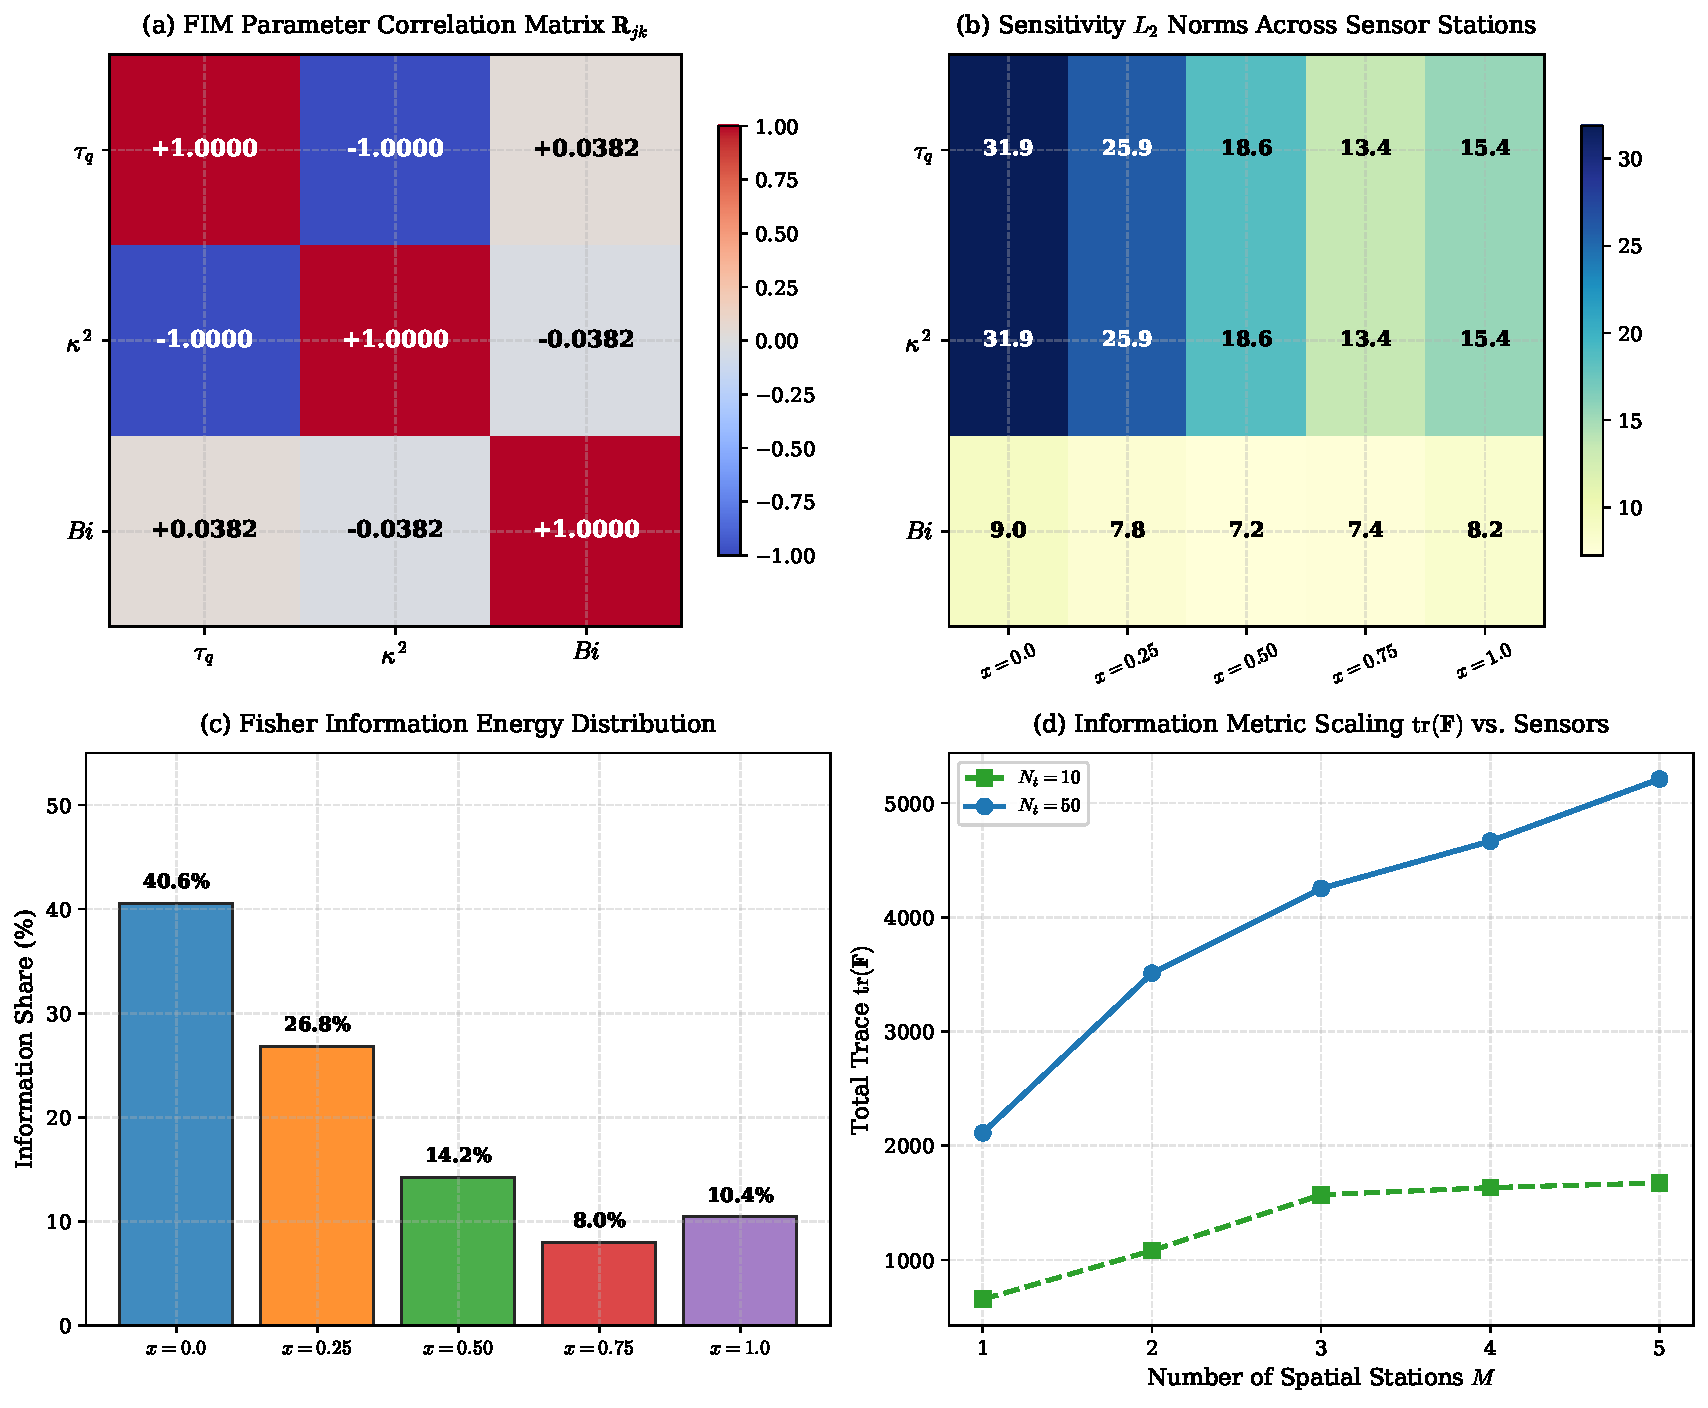
\includegraphics[width=\textwidth]{figures/fig6_sensitivity_heatmap_and_partition.pdf}
\caption{Fisher Information Matrix parameter correlation heatmap and multi-sensor information partition: (a) Parameter correlation matrix $\mathbf{R}_{jk} = F_{jk}/\sqrt{F_{jj}F_{kk}}$, displaying exact collinear anti-correlation $\rho(\tau_q, \kappa^2) = -1.0000$ and weak coupling with Biot number ($\rho = \pm 0.0382$). (b) Sensitivity $L_2$ norm distribution matrix across five sensor stations $x \in \{0.0, 0.25, 0.50, 0.75, 1.0\}$, showing uniform non-Fourier sensitivity norms. (c) Fisher information energy partition across sensor stations, demonstrating that front-face monitoring captures $40.6\%$ of total information energy while rear face captures $10.4\%$. (d) Information metric scaling $\operatorname{tr}(\mathbf{F})$ versus number of sensor stations $M \in \{1, \dots, 5\}$ for sampling rates $N_t = 10$ and $N_t = 50$.}
\label{fig:fig6}
\end{figure}

\subsection{Invariance Metrics Across Biot Numbers}

Table~\ref{tab:heatloss_sweep} and Figure~\ref{fig:fig7} summarize the collinearity and conditioning metrics across twelve Biot numbers ($Bi \in [0.001, 0.5]$), consistent with multi-parameter inverse estimation analyses~\cite{kovacs2015generalized,lapka2020development,nishi2020effect}. Across all evaluated cooling rates, the correlation coefficient between relaxation and nonlocal sensitivities is $\rho \equiv -1.0000000000$, with the defect $|1 + \rho| \le 2.22 \times 10^{-16}$ resting at the IEEE 754 double-precision floor (Figure~\ref{fig:fig7}(a)). The normalized residual norm $R_J = \|J_{\tau_q} + J_{\kappa^2}\| / \|J_{\tau_q}\| \approx (5.37 - 8.11) \times 10^{-9}$ matches the finite-difference discretization floor; step-size tests in 50-digit precision show that $R_J$ converges quadratically as $O(h^2)$, reaching $1.24 \times 10^{-14}$ at $h = 10^{-8}$ and $1.36 \times 10^{-18}$ at $h = 10^{-10}$. The corresponding Laplace-domain analytic-differentiation channel (Section~\ref{sec:sensitivity_landscapes}) reduces the same residual to zero to within the double-precision unit roundoff.

As shown in Figure~\ref{fig:fig7}(b), both the 2-parameter Fisher condition number $\operatorname{cond}(F_{2\times 2})$ and the 3-parameter condition number $\operatorname{cond}(F_{3\times 3})$ stay level at $10^{16}$--$10^{17}$, corresponding to the floating-point singularity floor for a matrix that is mathematically non-invertible. The analytical condition number at $B = 1$ is infinite; every finite value reported here is a numerical floor of the evaluation channel, not a finite physical conditioning.

\begin{table}[htbp]
\centering
\caption{Systematic parameter sweep across Biot numbers at Fourier resonance ($B = 1.0$): Collinearity metrics, singular spectrum $(\sigma_1, \sigma_2, \sigma_3)$, and Fisher condition numbers.}
\label{tab:heatloss_sweep}
\resizebox{\textwidth}{!}{
\begin{tabular}{cccccccccc}
\toprule
Biot Number $Bi$ & $\|J_{\tau_q}\|$ & $\|J_{Bi}\|$ & $\rho$ & $|1 + \rho|$ & $R_J$ & $\sigma_1$ & $\sigma_2$ & $\sigma_3$ & $\operatorname{cond}(F_{3\times 3})$ \\
\midrule
0.000 & 22.431 & 13.807 & $-1.0000000000$ & $1.11\times 10^{-16}$ & $5.37\times 10^{-9}$ & 31.82 & 13.57 & $7.37\times 10^{-8}$ & $1.86\times 10^{17}$ \\
0.001 & 22.421 & 13.779 & $-1.0000000000$ & $1.11\times 10^{-16}$ & $5.37\times 10^{-9}$ & 31.81 & 13.55 & $7.35\times 10^{-8}$ & $1.87\times 10^{17}$ \\
0.002 & 22.412 & 13.751 & $-1.0000000000$ & $2.22\times 10^{-16}$ & $5.38\times 10^{-9}$ & 31.79 & 13.52 & $7.38\times 10^{-8}$ & $1.86\times 10^{17}$ \\
0.005 & 22.382 & 13.666 & $-1.0000000000$ & $0.00\times 10^{-16}$ & $5.38\times 10^{-9}$ & 31.75 & 13.44 & $7.36\times 10^{-8}$ & $1.86\times 10^{17}$ \\
0.010 & 22.333 & 13.527 & $-1.0000000000$ & $2.22\times 10^{-16}$ & $5.39\times 10^{-9}$ & 31.68 & 13.30 & $7.36\times 10^{-8}$ & $1.85\times 10^{17}$ \\
0.020 & 22.237 & 13.253 & $-1.0000000000$ & $1.11\times 10^{-16}$ & $5.40\times 10^{-9}$ & 31.54 & 13.03 & $7.33\times 10^{-8}$ & $1.85\times 10^{17}$ \\
0.050 & 21.953 & 12.470 & $-1.0000000000$ & $0.00\times 10^{-16}$ & $5.41\times 10^{-9}$ & 31.13 & 12.27 & $7.25\times 10^{-8}$ & $1.84\times 10^{17}$ \\
0.100 & 21.502 & 11.287 & $-1.0000000000$ & $1.11\times 10^{-16}$ & $5.48\times 10^{-9}$ & 30.47 & 11.11 & $7.16\times 10^{-8}$ & $1.81\times 10^{17}$ \\
0.150 & 21.074 & 10.237 & $-1.0000000000$ & $0.00\times 10^{-16}$ & $5.53\times 10^{-9}$ & 29.86 & 10.07 & $7.09\times 10^{-8}$ & $1.77\times 10^{17}$ \\
0.200 & 20.666 & 9.304 & $-1.0000000000$ & $1.11\times 10^{-16}$ & $8.11\times 10^{-9}$ & 29.27 & 9.15 & $1.10\times 10^{-7}$ & $7.05\times 10^{16}$ \\
0.300 & 19.903 & 7.731 & $-1.0000000000$ & $2.22\times 10^{-16}$ & $5.65\times 10^{-9}$ & 28.18 & 7.60 & $6.82\times 10^{-8}$ & $1.71\times 10^{17}$ \\
0.500 & 18.548 & 5.462 & $-1.0000000000$ & $1.11\times 10^{-16}$ & $5.81\times 10^{-9}$ & 26.25 & 5.35 & $6.50\times 10^{-8}$ & $1.63\times 10^{17}$ \\
\bottomrule
\end{tabular}
}
\end{table}

\begin{figure}[htbp]
\centering
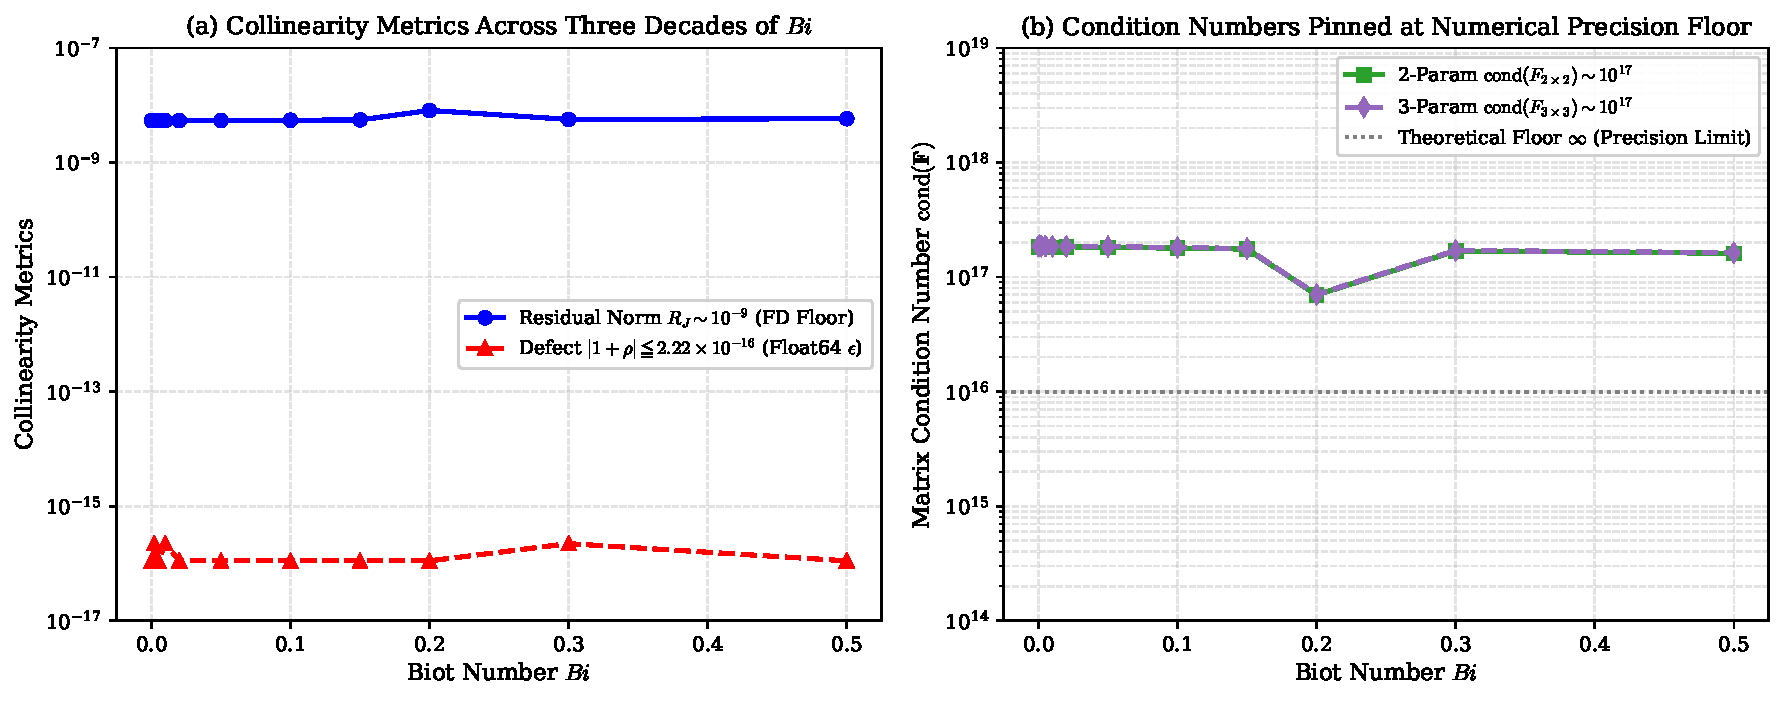
\includegraphics[width=\textwidth]{figures/fig7_invariance_metrics_vs_biot.pdf}
\caption{Collinearity and conditioning invariance metrics across Biot numbers ($Bi \in [0.001, 0.50]$): (a) Collinearity metrics across Biot numbers: residual norm $R_J \sim 10^{-9}$ (finite-difference truncation floor) and correlation defect $|1+\rho| \le 2.22 \times 10^{-16}$ (IEEE 754 double-precision floor). (b) 2-parameter and 3-parameter Fisher Information condition numbers pinned horizontally at the floating-point singularity floor ($10^{16}$--$10^{17}$; the analytical value at $B=1$ is infinite).}
\label{fig:fig7}
\end{figure}

\subsection{Singularity Canyon Topography and Observable Subspace Conditioning}

Figure~\ref{fig:fig8} presents the topography of the Singularity Canyon and examines the conditioning of the observable subspace in the 3-parameter setting $\bm{p} = (\tau_q, \kappa^2, Bi)^\top$. Figure~\ref{fig:fig8}(a) displays the surface $\log_{10}\operatorname{cond}(\mathbf{F}_{3\times 3})(B, Bi)$, computed from the three-parameter Jacobian $\bm{J} = [\bm{J}_{\tau_q}, \bm{J}_{\kappa^2}, \bm{J}_{Bi}]$, across the domain $(B, Bi) \in [0.5, 1.5] \times [0.0, 0.5]$. A steep, narrow canyon is centered along $B = 1$, where the analytical condition number is infinite and the computed value saturates at the IEEE 754 singularity floor of the evaluation channel ($10^{16}$--$10^{17}$ across all Biot numbers). Figure~\ref{fig:fig8}(b) shows the iso-conditioning contours: the singular canyon forms a straight vertical trench aligned with the resonance line $B = 1$ (black dashed line), indicating that boundary heat loss does not shift or soften the singular corridor.

\begin{figure}[htbp]
\centering
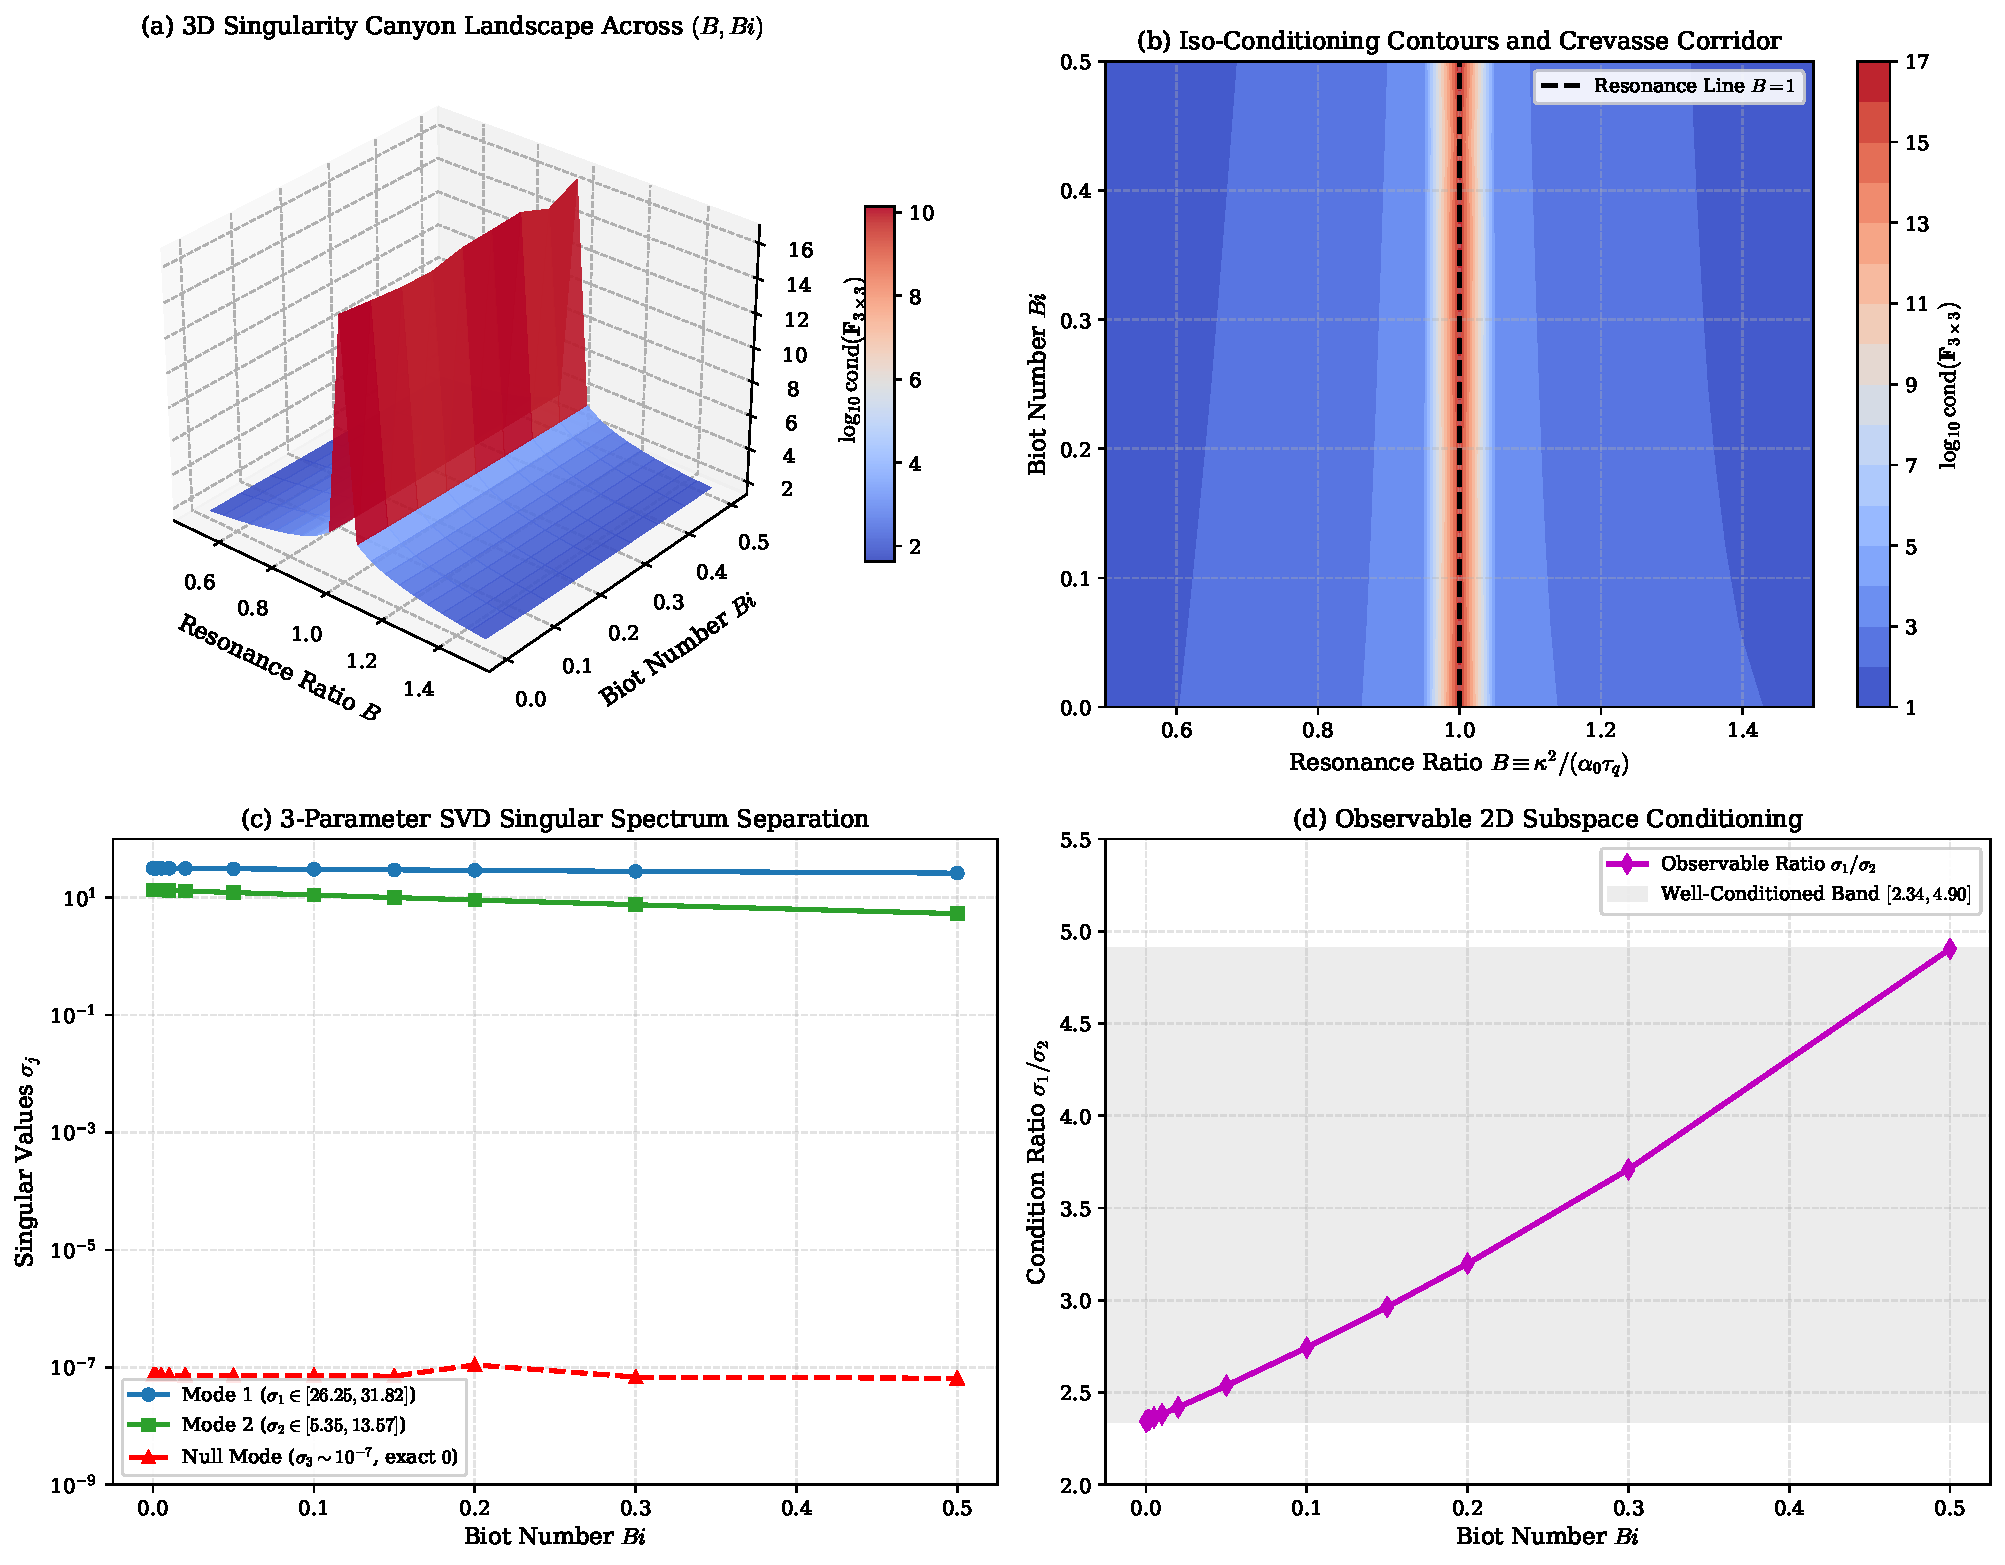
\includegraphics[width=\textwidth]{figures/fig8_3d_singularity_canyon_and_spectrum.pdf}
\caption{Singularity canyon topography and observable subspace conditioning: (a) 3D Fisher condition number surface $\log_{10}\operatorname{cond}(\mathbf{F}_{3\times 3})(B, Bi)$ over $(B, Bi) \in [0.5, 1.5] \times [0.0, 0.5]$, illustrating the sharp resonance crevasse pinned along $B = 1$ across all Biot numbers; at $B = 1$ the analytical condition number is infinite and the plotted value is the double-precision singularity floor of the evaluation channel. (b) Iso-conditioning contours and crevasse corridor in the $(B, Bi)$ plane with dashed resonance line $B = 1$. (c) 3-Parameter SVD spectrum showing complete modal separation between the physical observable subspace ($\sigma_1 \in [26.25, 31.82]$, $\sigma_2 \in [5.35, 13.57]$) and the structural null singularity ($\sigma_3 \sim 10^{-8}$ in the time-domain finite-difference channel; the analytical value is $\sigma_3 \equiv 0$, confirmed to below the double-precision unit roundoff by the Laplace-domain analytic-differentiation channel). (d) Condition ratio of the observable 2D subspace $\sigma_1/\sigma_2 \in [2.34, 4.90]$ across Biot numbers.}
\label{fig:fig8}
\end{figure}

Singular Value Decomposition of the Jacobian $\bm{J}$ reveals clear separation between observable modes and the null space (Figure~\ref{fig:fig8}(c)). The first mode ($\sigma_1 \in [26.25, 31.82]$) corresponds to early-time thermal diffusion through the bulk. The second mode ($\sigma_2 \in [5.35, 13.57]$) reflects surface heat loss in the cooling tail. The condition ratio of this observable 2D subspace remains moderate (Figure~\ref{fig:fig8}(d)):
\begin{equation}
\frac{\sigma_1}{\sigma_2} \in [2.34, 4.90],
\end{equation}
confirming that the observable subspace is well-conditioned. Because the structural null vector $\bm{v}_{\mathrm{null}} = (1, 1, 0)^\top$ has no projection along $Bi$ ($\bm{c}_{Bi}^\top \bm{v}_{\mathrm{null}} = 0$), $Bi$ is an estimable parametric functional on the observable range space $\mathcal{R}(\bm{F})$. Evaluating the generalized Cramér--Rao bound from the Moore--Penrose pseudoinverse $(\bm{J}^\top \bm{J})^\dagger$ of the three-parameter Fisher matrix (Eq.~\eqref{eq:se_bi_def}) yields $\operatorname{SE}(\hat{Bi}) / \sigma_n = \sqrt{[(\bm{J}^\top \bm{J})^\dagger]_{33}} = 0.1243$ for the rear-face sampling ($N_t = 50$, $Bi = 0.10$); this value is reported in Table~\ref{tab:crlb_analysis}. Under $1.0\%$ measurement noise ($\sigma_n = 10^{-2}$), this gives $\operatorname{SE}(\hat{Bi}) \approx 1.24 \times 10^{-3}$, representing a $1.24\%$ relative uncertainty on $Bi = 0.10$ (and $0.12\%$ uncertainty under $0.1\%$ noise). Because $\bm{c}_{\tau_q}$ and $\bm{c}_{\kappa^2}$ are not orthogonal to the null space, the corresponding generalized bounds do not exist at $B = 1$ and are reported as not estimable.

In contrast, the third singular mode corresponds to the structural null vector $\bm{v}_{\mathrm{null}} = (1, 1, 0)^\top$ with direction cosine $1.000000$. In the time-domain finite-difference channel (relative step $h_{\mathrm{rel}} = 10^{-4}$, i.e., $\Delta\tau_q = \Delta\kappa^2 = 2 \times 10^{-6}$) the computed value is $\sigma_3 \approx 7.3 \times 10^{-8}$; under high-precision variable step sizes it drops to $10^{-18}$, and in the Laplace-domain analytic-differentiation channel it is zero to below the double-precision unit roundoff. The analytical singular value is therefore identically zero, and every non-zero computed value is a truncation or round-off floor of the corresponding evaluation channel. Because boundary cooling acts along an orthogonal coordinate, it provides zero projection onto this null vector, leaving the parameter degeneracy between $\tau_q$ and $\kappa^2$ unregularized.

\subsection{Near-Resonance Behavior and Asymptotic Scaling}
\label{sec:near_resonance}

Figure~\ref{fig:fig9} analyzes the near-resonance behavior and examines the two-sided linear asymptotic power law as the resonance parameter $B \equiv \kappa^2 / (\alpha_0 \tau_q)$ traverses $[0.5, 1.5]$ for $Bi \in \{0.00, 0.05, 0.20\}$. Away from resonance, the condition number is modest ($\sim 10^1$ to $10^2$). However, as $B \to 1$, $\operatorname{cond}(F)$ grows sharply, forming a deep condition canyon (Figure~\ref{fig:fig9}(a)).

\paragraph{Analytical Taylor expansion and power-law verification}
Let $\delta \equiv B - 1$. Expanding $m(s)$ and $\mu(s)$ in powers of $\delta$:
\begin{align}
m(s) &= \sqrt{s} \left[ 1 - \frac{1}{2}\left(\frac{\tau_q s}{1 + \tau_q s}\right) \delta + O(\delta^2) \right], \\
m(s)\mu(s) &= \sqrt{s} \left[ 1 + \frac{1}{2}\left(\frac{\tau_q s}{1 + \tau_q s}\right) \delta + O(\delta^2) \right].
\end{align}
Because both the bulk propagation factor and the surface conductivity factor depart linearly with $\delta$, the sensitivity collinearity defect satisfies $\bm{J}_{\tau_q} + \bm{J}_{\kappa^2} = \bm{g}(t; Bi) \, \delta + O(\delta^2)$ (dimensionless parameterization). Consequently, the smallest singular value of the three-parameter Jacobian follows the linear power law:
\begin{equation}
\sigma_{\min}(B) \approx C(Bi) |B - 1|^{1.0},
\label{eq:scaling_law}
\end{equation}
where $C(Bi) \in [1.348, 1.464]$ across $Bi \in [0.0, 0.5]$. The mean scaling prefactor $C(Bi)$ decreases monotonically from $1.464$ under adiabatic conditions ($Bi = 0$) to $1.348$ under stronger convection ($Bi = 0.50$) (Figure~\ref{fig:fig9}(c)). In comparison, branch-specific two-sided linear regressions of the smallest singular value at baseline $Bi = 0.10$ (Figure~\ref{fig:fig9}(b)) confirm:
\begin{itemize}
    \item For $B < 1$ ($B \in [0.90, 0.999]$): log-log exponent $1.0059 \pm 0.0022$ ($R^2 = 0.99998$), with branch-specific slope $C = 1.481$.
    \item For $B > 1$ ($B \in [1.001, 1.10]$): log-log exponent $0.9986 \pm 0.0002$ ($R^2 = 1.00000$), with branch-specific slope $C = 1.426$.
\end{itemize}
We distinguish the mean scaling prefactor $C(Bi) \in [1.348, 1.464]$ averaged across $Bi$ from these branch-specific regression slopes ($C = 1.481$ for $B < 1$ and $C = 1.426$ for $B > 1$ at $Bi = 0.10$). Regressing the smallest singular value of the two-parameter $(\tau_q, \kappa^2)$ subsystem instead gives $C = 1.512$ and $C = 1.436$ respectively, confirming that the two definitions of $\sigma_{\min}$ agree to within $2\%$. Figure~\ref{fig:fig9}(d) examines the relative residual of the single-prefactor linear approximation across the scanned corridor. Over the regression range $|B - 1| \le 0.10$ the linear asymptote reproduces the smallest singular value to within $3.3\%$ on the $B < 1$ branch and $0.7\%$ on the $B > 1$ branch; outside that range the residual grows (to $6.3\%$ at $|B-1| = 0.2$ and $34\%$ at $|B-1| = 0.5$ on the left branch), as expected for an asymptotic law.

\begin{figure}[htbp]
\centering
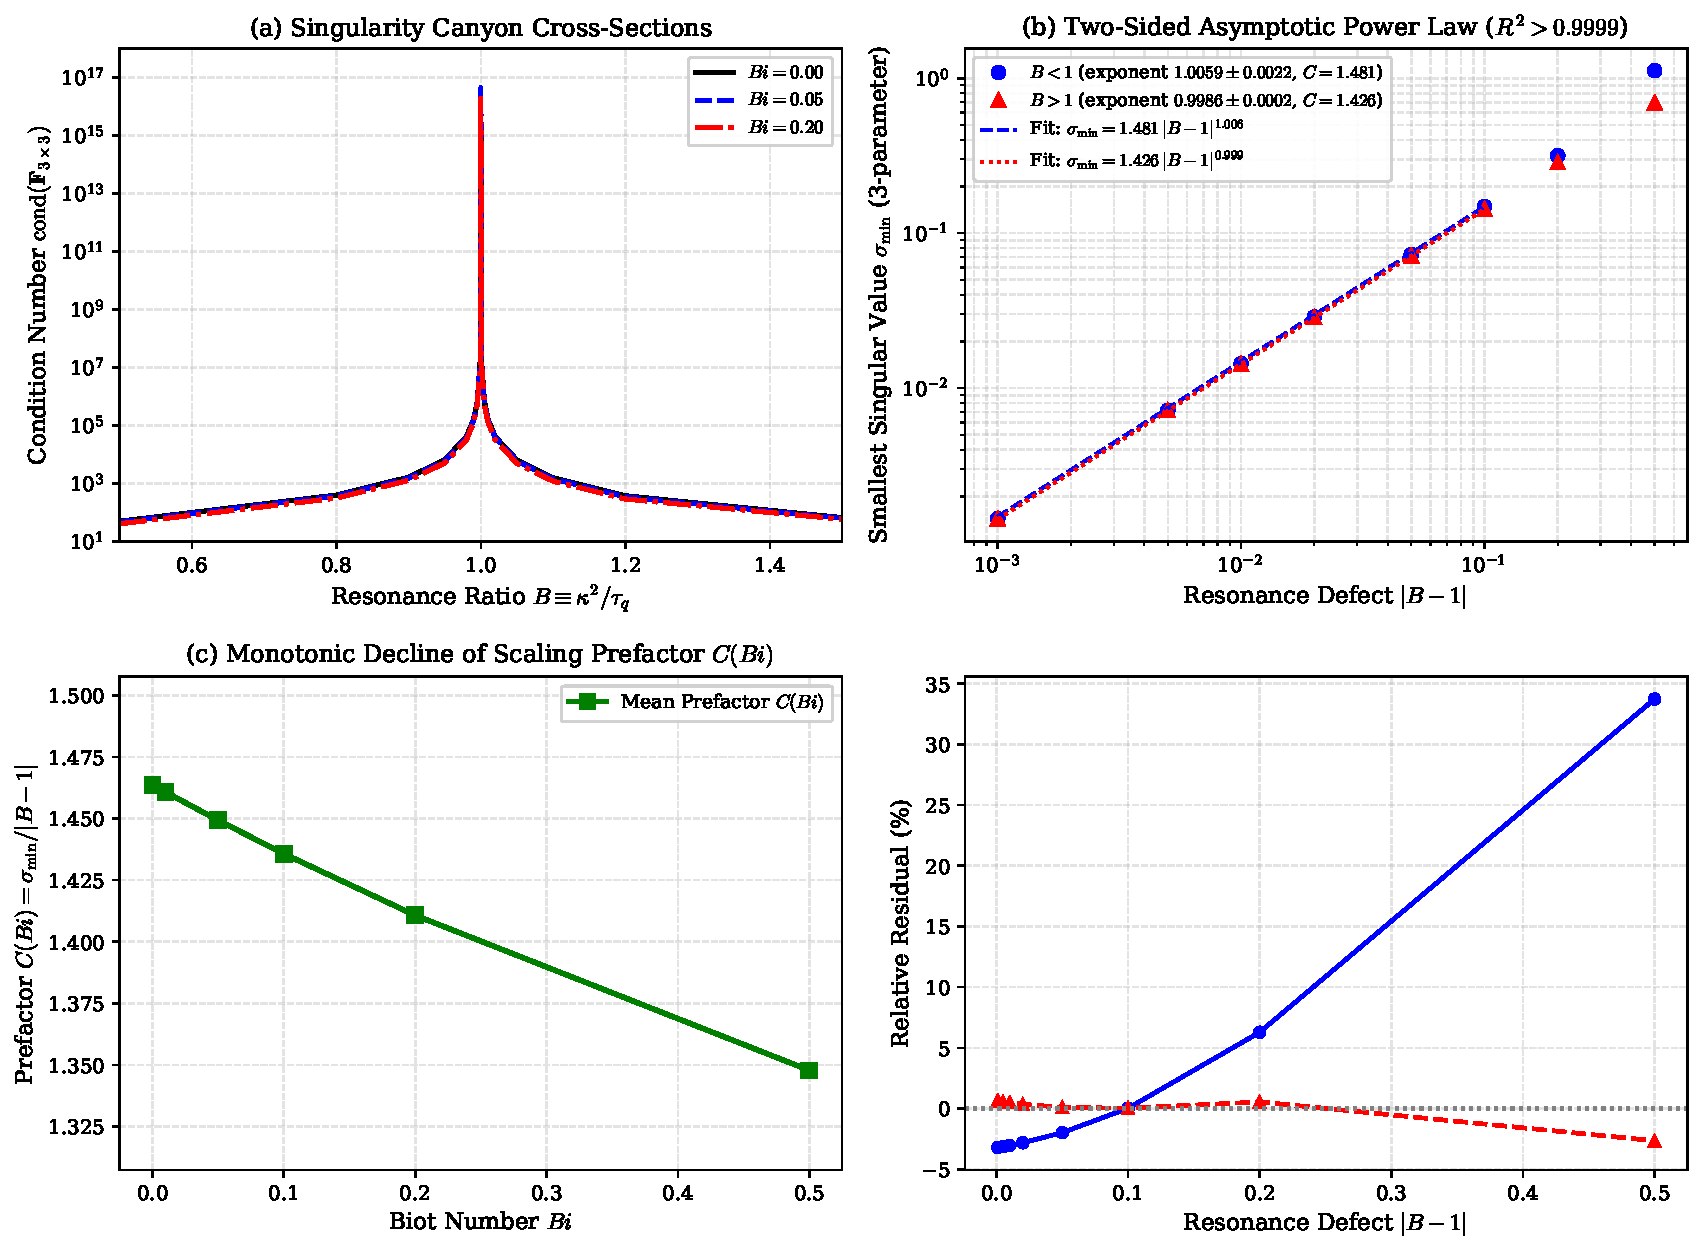
\includegraphics[width=\textwidth]{figures/fig9_near_resonance_scaling.pdf}
\caption{Near-resonance scaling and two-sided linear power law: (a) Cross-sectional profiles of the condition number canyon centered at $B = 1.0$ for $Bi \in \{0.00, 0.05, 0.20\}$. (b) Two-sided asymptotic log-log power-law regression of the smallest singular value of the three-parameter Jacobian, $\sigma_{\min} \approx C(Bi)|B-1|^{1.0}$ ($R^2 > 0.9999$) at baseline $Bi = 0.10$, showing branch-specific slopes $C = 1.481$ (left branch, exponent $1.0059 \pm 0.0022$) and $C = 1.426$ (right branch, exponent $0.9986 \pm 0.0002$). (c) Monotonic decline of the mean scaling prefactor $C(Bi) = \operatorname{mean}_B(\sigma_{\min}/|B-1|)$ across Biot numbers from $1.464$ at $Bi = 0$ to $1.348$ at $Bi = 0.50$. (d) Relative residual of the single-prefactor linear asymptote across the scanned corridor $|B-1| \le 0.5$; the branch regressions are fitted over $|B-1| \le 0.10$.}
\label{fig:fig9}
\end{figure}

\subsection{Cramér--Rao Lower Bounds and Parameter Estimation Precision}

To assess practical parameter estimation limits, we evaluate the Cramér--Rao lower bounds in the full three-parameter estimation space $\bm{p} = (\tau_q, \kappa^2, Bi)^\top$, using the sensitivity Jacobian $\bm{J} = [\bm{J}_{\tau_q} \; \bm{J}_{\kappa^2} \; \bm{J}_{Bi}]$ and the Fisher matrix $\bm{F} = \sigma_n^{-2} \bm{J}^\top \bm{J}$ of Eq.~\eqref{eq:fim_def}; every Jacobian column is obtained by analytic differentiation of the closed-form transfer function. Near resonance ($B = 0.99$) the Fisher matrix is non-singular and the ordinary CRLB applies, while at exact resonance ($B = 1$) it is structurally singular and the generalized (Moore--Penrose) bound of Eq.~\eqref{eq:generalized_crlb} applies. Table~\ref{tab:crlb_analysis} and Figure~\ref{fig:fig10} summarize the critical corridor half-width $|B - 1|_{\mathrm{crit}}$ needed to achieve a $10\%$ relative parameter standard error ($\operatorname{SE}(\hat{\tau}_q) / \tau_{q,0} \le 0.10$ with baseline $\tau_{q,0} = 0.02$) across measurement geometries, temporal sampling sizes $N_t$, and noise levels $\sigma_n \in \{0.1\%, 0.5\%, 1.0\%\}$. All values quoted below are listed in Table~\ref{tab:crlb_analysis}.

\begin{table}[htbp]
\centering
\caption{Three-parameter Cramér--Rao Lower Bound (CRLB) estimation precision: critical near-resonance corridor half-width $|B - 1|_{\mathrm{crit}}$ required to achieve $\operatorname{SE}(\hat{\tau}_q) / \tau_{q,0} \le 0.10$ across observation configurations and noise floors, evaluated at $B = 0.99$ and $Bi = 0.10$ with the Fisher matrix $\bm{F} = \sigma_n^{-2}\bm{J}^\top\bm{J}$ of the three-parameter Jacobian $\bm{J} = [\bm{J}_{\tau_q}, \bm{J}_{\kappa^2}, \bm{J}_{Bi}]$. The "Singular" column uses the smallest singular value $\sigma_3$; the "Param" column uses the marginal $\tau_q$ coordinate bound. At exact resonance ($B = 1$) the Fisher matrix is singular and only $Bi$ admits a finite generalized bound ($\operatorname{SE}(\hat{Bi})/\sigma_n = 0.1243$ for rear-face sampling with $N_t = 50$).}
\label{tab:crlb_analysis}
\resizebox{\textwidth}{!}{
\begin{tabular}{lcccccc}
\toprule
Sensor Configuration & Sampling $N_t$ & Noise Level $\sigma_n$ & $\sigma_3 / |B-1|$ & $\operatorname{SE}(\hat{\tau}_q)/\sigma_n \cdot |B-1|$ & $|B-1|_{\mathrm{crit}}$ (Param) & $|B-1|_{\mathrm{crit}}$ (Singular) \\
\midrule
Rear-face only ($x = 1.0$) & 10 & 0.1\% & 1.438 & 0.491 & 0.246 & 0.348 \\
Rear-face only ($x = 1.0$) & 10 & 0.5\% & 1.438 & 0.491 & 1.228 & 1.739 \\
Rear-face only ($x = 1.0$) & 10 & 1.0\% & 1.438 & 0.491 & 2.455 & 3.478 \\
\midrule
Rear-face only ($x = 1.0$) & 50 & 0.1\% & 3.858 & 0.183 & 0.092 & 0.130 \\
Rear-face only ($x = 1.0$) & 50 & 0.5\% & 3.858 & 0.183 & 0.459 & 0.648 \\
Rear-face only ($x = 1.0$) & 50 & 1.0\% & 3.858 & 0.183 & 0.917 & 1.296 \\
\midrule
Rear-face only ($x = 1.0$) & 100 & 0.1\% & 5.482 & 0.129 & 0.065 & 0.091 \\
Rear-face only ($x = 1.0$) & 100 & 0.5\% & 5.482 & 0.129 & 0.323 & 0.456 \\
Rear-face only ($x = 1.0$) & 100 & 1.0\% & 5.482 & 0.129 & 0.645 & 0.912 \\
\midrule
Front + Rear ($x = 0, 1$) & 50 & 0.1\% & 23.58 & 0.030 & 0.015 & 0.021 \\
Front + Rear ($x = 0, 1$) & 50 & 0.5\% & 23.58 & 0.030 & 0.075 & 0.106 \\
Front + Rear ($x = 0, 1$) & 50 & 1.0\% & 23.58 & 0.030 & 0.151 & 0.212 \\
\midrule
Multi-location (5 stations) & 50 & 0.1\% & 28.17 & 0.025 & 0.013 & 0.018 \\
Multi-location (5 stations) & 50 & 0.5\% & 28.17 & 0.025 & 0.063 & 0.089 \\
Multi-location (5 stations) & 50 & 1.0\% & 28.17 & 0.025 & 0.126 & 0.178 \\
\bottomrule
\end{tabular}
}
\end{table}

\begin{figure}[htbp]
\centering
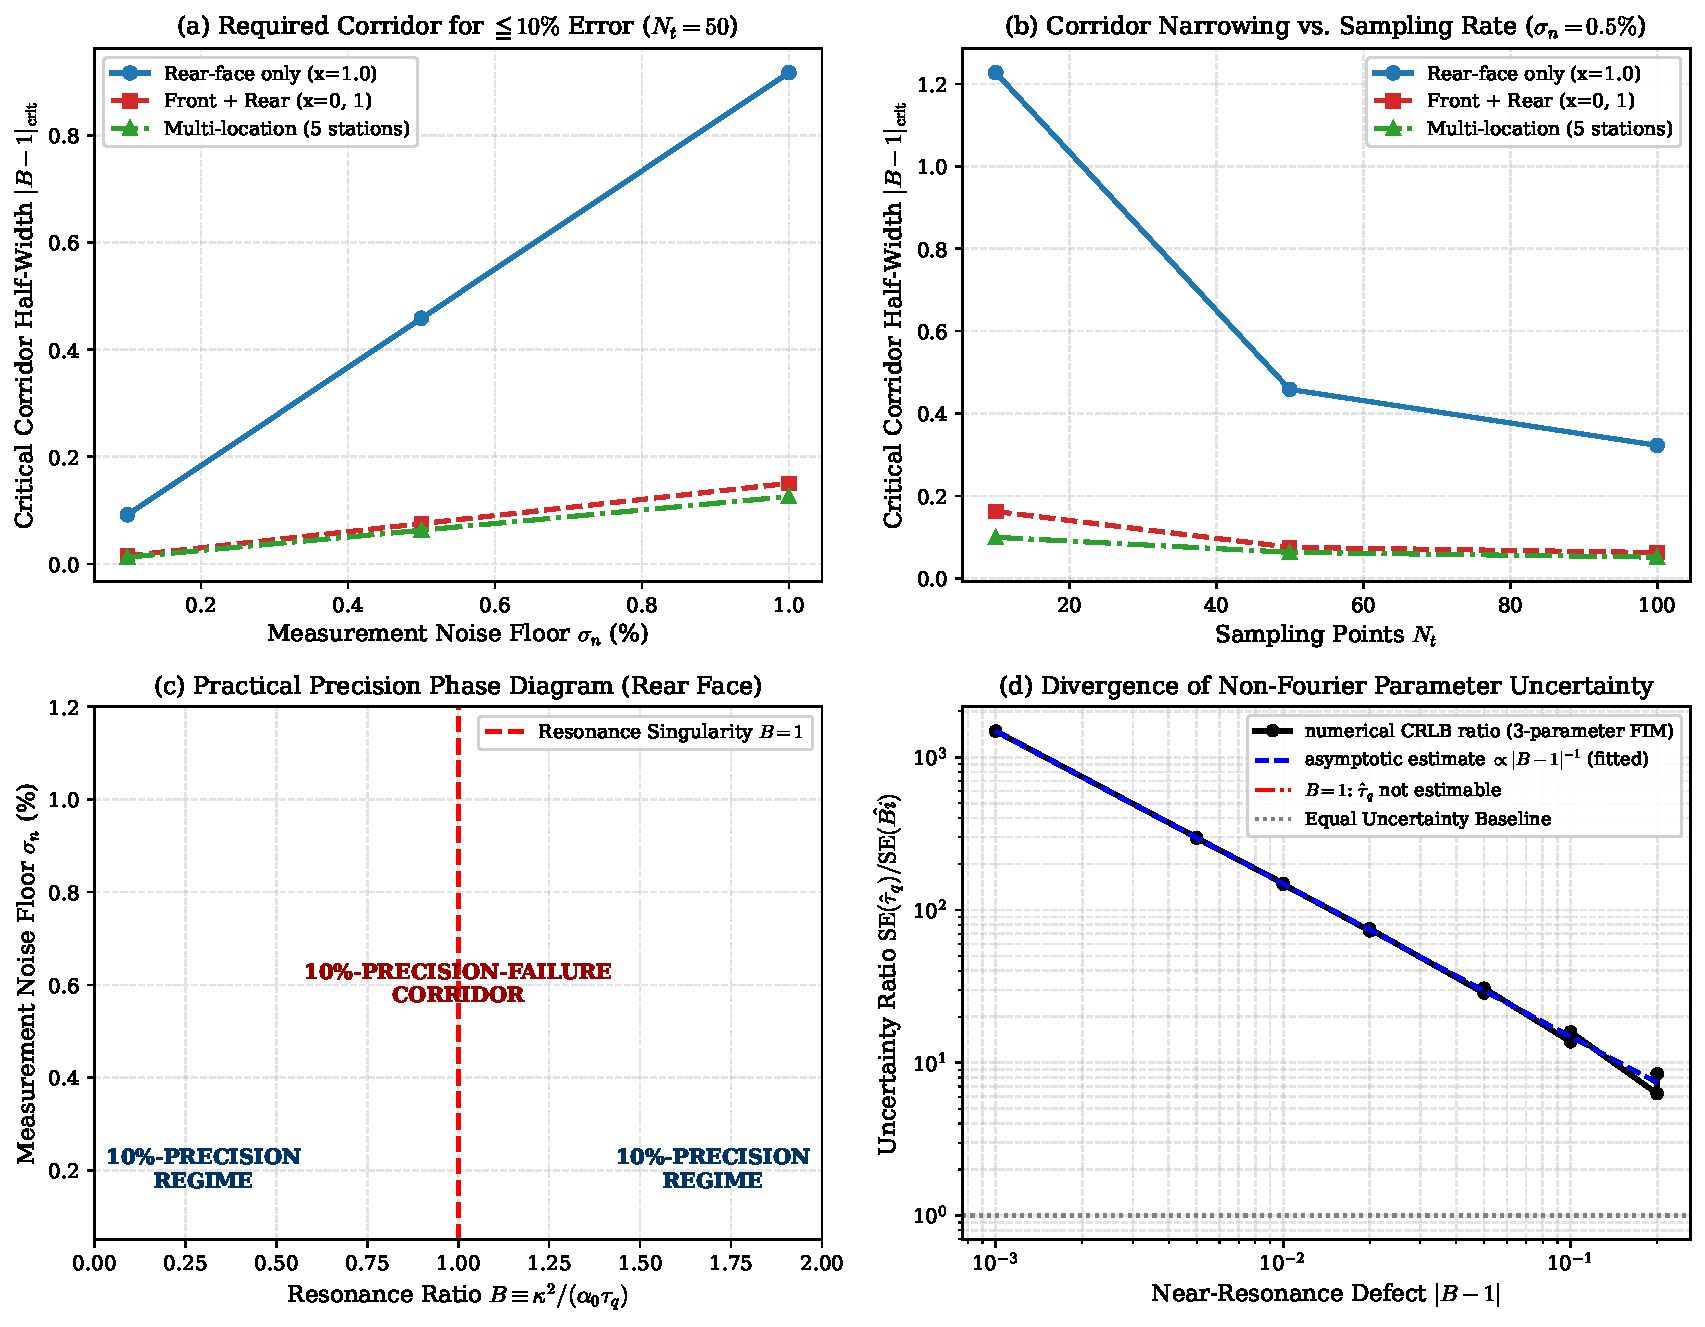
\includegraphics[width=\textwidth]{figures/fig10_crlb_identifiability_maps.pdf}
\caption{Cramér--Rao Lower Bound (CRLB) identifiability maps and practical precision phase diagrams: (a) Critical near-resonance corridor half-width $|B-1|_{\mathrm{crit}}$ required for $\operatorname{SE}(\hat{\tau}_q)/\tau_{q,0} \le 10\%$ versus measurement noise floor $\sigma_n \in [0.1\%, 1.0\%]$ ($N_t = 50$). (b) Corridor narrowing under increasing temporal sampling density $N_t \in [10, 100]$ at $\sigma_n = 0.5\%$. (c) Practical precision phase diagram in the $(B, \sigma_n)$ plane demarcating the 10\%-precision-failure corridor from the 10\%-precision regime for rear-face monitoring; the corridor boundary is computed from the three-parameter CRLB analysis. (d) Divergence of the non-Fourier parameter uncertainty ratio $\operatorname{SE}(\hat{\tau}_q)/\operatorname{SE}(\hat{Bi})$ as resonance is approached: markers are the numerical ratio computed directly from the three-parameter Fisher matrix (rear face, $N_t = 50$, $Bi = 0.10$), and the dashed curve is the asymptotic $1/|B-1|$ estimate fitted to the well-conditioned part of the same scan. At $B = 1$ the Fisher matrix is singular and $\hat{\tau}_q$ is not estimable.}
\label{fig:fig10}
\end{figure}

Several points emerge from this analysis:
\begin{enumerate}
    \item \textit{Origin of Coarse-Sampling Thresholds:} The values $|B - 1|_{\mathrm{crit}} \approx 0.35$ (0.1\% noise) and $3.48$ (1.0\% noise) stem from a sparse 10-point rear-face sampling evaluating parameter uncertainty along the principal singular mode ($\sigma_n / (0.10 C \tau_{q,0})$).
    \item \textit{Influence of Sampling Density ($N_t = 50$):} With denser sampling ($N_t = 50$, Figure~\ref{fig:fig10}(a)), the sensitivity norm increases roughly as $\sqrt{N_t}$, contracting the critical corridor for parameter $\tau_q$ to $|B - 1|_{\mathrm{crit}} \approx 0.092$ under $0.1\%$ noise and $0.917$ under $1.0\%$ noise. At $1.0\%$ noise, simultaneous parameter estimation remains challenging across $B \in [0.083, 1.917]$ (Figure~\ref{fig:fig10}(c)).
    \item \textit{Temporal Sampling Progression ($N_t$):} Figure~\ref{fig:fig10}(b) illustrates the narrowing of the corridor as $N_t$ rises from 10 to 100, following an asymptotic $\sim 1/\sqrt{N_t}$ contraction.
    \item \textit{Dual-Surface Monitoring ($x = 0$ and $x = 1$):} Recording both front and rear surfaces substantially increases the sensitivity norm ($\sigma_3/|B-1| \approx 23.6$), reducing the corridor to $|B - 1|_{\mathrm{crit}} \approx 0.015$ (0.1\% noise) and $0.151$ (1.0\% noise).
    \item \textit{Uncertainty Ratio Divergence:} Figure~\ref{fig:fig10}(d) shows that while the Biot number standard error stays bounded ($\operatorname{SE}(\hat{Bi})/\sigma_n = 0.1243$, i.e. $\operatorname{SE}(\hat{Bi}) \approx 1.24 \times 10^{-3}$ under $1.0\%$ noise), the non-Fourier uncertainty diverges: the numerically computed ratio $\operatorname{SE}(\hat{\tau}_q)/\operatorname{SE}(\hat{Bi})$ follows the fitted asymptotic $1/|B-1|$ law over the well-conditioned part of the scan, and $\hat{\tau}_q$ ceases to be estimable at $B = 1$.
\end{enumerate}

\section{Experimental Implications and Regularization}

The heat-loss invariance demonstrated here carries direct implications for laser flash thermal metrology and non-Fourier materials characterization.

\subsection{Standard Flash Data Reduction and Scope of ASTM E1461}

ASTM E1461-13(2022)~\cite{astm2022standard} is a standard test method for flash-method thermal-diffusivity measurement: it prescribes the measurement geometry, the pulse and data-reduction procedure, and the analytical heat-loss and finite-pulse corrections (developed in the literature, e.g., by Cowan~\cite{cowan1963pulse}, Cape and Lehman~\cite{cape1963temperature}, Heckman~\cite{heckman1973finite}, and Clark and Taylor~\cite{clark1975radiation}). It does not prescribe an inverse-identification algorithm for non-Fourier constitutive parameters. In practice, flash-instrument software typically implements non-linear regression of full thermograms to analytical or numerical transfer functions that incorporate boundary heat loss and finite pulse duration~\cite{baba2001improvement,blumm2002improvement,sundar2025thermal,blumm2025laser}. The present study is an independent theoretical analysis of the identifiability of such a regression within the Guyer--Krumhansl model; it does not rely on, extend, or modify the standard itself. When researchers extend laser flash testing to candidate non-Fourier materials, the metrological question arises whether incorporating linear convective and radiative boundary heat loss allows the simultaneous inverse identification of Guyer--Krumhansl constitutive parameters $(\tau_q, \kappa^2)$. Theorem~1 proves mathematically that for the linear 1D Guyer--Krumhansl model, incorporating linear Robin boundary heat loss does not remove the structural null direction associated with $\tau_q$ and $\kappa^2$ at exact resonance ($B = 1$). Because both the bulk propagation operator and the dynamic surface thermal conductivity collapse simultaneously to Fourier diffusion at $B = 1$, any parameter combination satisfying $\kappa^2 = \alpha_0 \tau_q$ yields a transient thermogram that is mathematically indistinguishable from that of a classical Fourier material with the same Biot numbers. Consequently, a Fourier-model fit can reproduce the resonant GK thermogram with zero model discrepancy under the stated mathematical assumptions, providing no indication that the underlying transport involves non-zero relaxation and nonlocal length scales satisfying $\kappa^2 = \alpha_0 \tau_q$.

\subsection{Specimen Thickness Scaling and Nonlocal Size Effects}
\label{sec:thickness}

For a homogeneous bulk material with constant physical properties, the resonance ratio $B \equiv \kappa^2 / (\alpha_0 \tau_q)$ is scale-invariant and independent of specimen thickness $L$. However, reducing $L$ shortens the diffusion timescale $t_{\mathrm{diff}} = L^2 / \alpha_0$, amplifying the dimensionless relaxation parameter $\hat{\tau}_q = \alpha_0 \tau_q / L^2$. The scaling suggests that reducing specimen thickness may amplify the sensitivity and could help move the estimation problem away from the ill-conditioned noise corridor; a direct numerical demonstration is outside the scope of the present fixed-geometry analysis and is left to future work. Furthermore, in nanolayers, thin films, and microscale heterostructures where boundary scattering induces size-dependent mean free paths ($\kappa = \kappa(L)$)~\cite{alvarez2007memory,guo2015phonon,minnich2012determining,cahill2014nanoscale,sellitto2016mesoscopic,sellitto2025nonlinear,zhu2017nonlocal}, specimen thickness directly tunes the constitutive parameter ratio away from unity ($B \ne 1$).

\subsection{Multi-Sensor Detection and Identifiability}

In photothermal and flash metrology, multi-sensor configurations (such as simultaneous front-face thermoreflectance and rear-face pyrometry~\cite{salazar2014extending}) are increasingly employed to decouple surface from bulk phenomena. As demonstrated by Emery et al.~\cite{emery2000uncertainties}, Fadale et al.~\cite{fadale1995two}, Dowding et al.~\cite{dowding1995estimation}, and {\L}apka et al.~\cite{lapka2020development}, optimal sensor placement maximizes the determinant of the Fisher Information Matrix. From Theorem~1, if $\theta_{\mathrm{GK}}(x, t; B=1) \equiv \theta_{\mathrm{Fourier}}(x, t)$ holds for all $x \in [0, 1]$ and all $t \ge 0$, then differentiating with respect to the constitutive parameters yields $\partial \theta / \partial \tau_q(x, t) = -\partial \theta / \partial \kappa^2(x, t)$ at every spatial point across the specimen (dimensionless parameterization). Stacking measurements from multiple sensors adds additional rows to the sensitivity matrix $\bm{J}$, but the two parameter columns remain strictly linearly dependent: $\bm{J}_{\tau_q} = -\bm{J}_{\kappa^2}$. Consequently, at exact resonance ($B = 1$) under the linear 1D model, multi-sensor monitoring cannot remove the structural rank deficiency ($\operatorname{rank}(\bm{J}) \le 2$ in the 3-parameter space $(\tau_q, \kappa^2, Bi)$). However, for near-resonant media ($B \ne 1$), our CRLB analysis (Table~\ref{tab:crlb_analysis}) demonstrates that multi-sensor configurations substantially improve near-resonance practical precision while leaving the exact-resonance structural null direction unchanged, amplifying the non-degenerate singular values and contracting the required noise corridor from $|B-1| \ge 0.917$ down to $|B-1| \ge 0.151$ under $1.0\%$ noise.

\subsection{Linear Robin Boundary Conditions versus Nonlinear Radiation}

Theorem~1 strictly applies to linear Robin boundary operators. While convective cooling and small-temperature-rise radiative cooling ($\theta / T_0 \ll 1$) conform to this assumption, high-temperature experiments subjected to full nonlinear Stefan--Boltzmann radiation ($q_{\mathrm{rad}} \propto T^4 - T_0^4$) generate surface harmonics that fall outside the linear transfer function framework. Similarly, operating at elevated laser pulse fluences may induce temperature-dependent thermal conductivity ($\lambda = \lambda(T)$) or volumetric heat capacity ($c = c(T)$). Nonlinear temperature-dependent transport would break the spatial invariance required for resonance, but evaluating whether such mechanisms provide parameter regularization would require a separate nonlinear identifiability analysis that is outside the scope of the present linear constitutive model~\cite{kovacs2020numerical,sellitto2025nonlinear,maillet2019review}.

\subsection{Limitations of the Present Analysis}
\label{sec:limitations}

The conclusions above are conditional on the modelling assumptions of the present study and should be read with the following limitations in mind.
\begin{enumerate}
    \item \textit{Model class.} Theorem~1 and all numerical results hold for the linear 1D Guyer--Krumhansl model with constant $\lambda_0$, $\tau_q$, $\kappa^2$ and linearized Robin boundary conditions (Eq.~\eqref{eq:h_eff_def}, valid for $\theta / T_0 \ll 1$) on a planar slab. Temperature-dependent coefficients, flux-dependent mean free paths, radial losses, full nonlinear Stefan--Boltzmann radiation, and non-causal constitutive extensions are outside this model class.
    \item \textit{Statistical assumptions.} The Cramér--Rao analysis assumes additive i.i.d. Gaussian noise with known standard deviation; correlated detector noise, baseline drift, and pulse-energy jitter are not propagated into the reported bounds. The study is theoretical and computational: no experimental measurements were performed, and implications for practice are model predictions.
    \item \textit{Fixed geometry.} The near-resonance and CRLB scans use fixed $\tau_{q,0} = 0.02$, $\kappa^2 = B\,\tau_{q,0}$, $\tau_\Delta = 0.04$ and unit thickness; thickness- and pulse-driven variations of the practical corridor (Section~\ref{sec:thickness}) require a separate parametric study.
\end{enumerate}

\section{Conclusions}

This study investigated whether convective and radiative boundary heat loss can regularize the Guyer--Krumhansl parameter identifiability singularity at Fourier resonance ($B \equiv \kappa^2 / (\alpha_0 \tau_q) = 1$), using analytical derivation in the Laplace domain and multi-tier numerical validation across $Bi \in [0.001, 0.5]$. The main quantitative findings are:

\begin{itemize}
    \item At $B = 1$, the GK field coincides identically with the classical Fourier field for all $x \in [0, 1]$, all $t \ge 0$, and all $Bi_0, Bi_L \ge 0$ (Theorem~1; numerical field residual at the $10^{-14}$ double-precision floor).
    \item The sensitivity collinearity $\partial \theta / \partial \tau_q = -\partial \theta / \partial \kappa^2$ holds for all $Bi$: correlation $\rho \equiv -1.0000000000$ and FIM null vector $\bm{v}_{\mathrm{null}} = (1, 1, 0)^\top$ with $\sigma_3 \equiv 0$.
    \item The observable 2D subspace is well-conditioned, $\sigma_1 / \sigma_2 \in [2.34, 4.90]$ across $Bi \in [0, 0.5]$.
    \item The Biot number remains estimable at $B = 1$ with $\operatorname{SE}(\hat{Bi})/\sigma_n = 0.1243$ (rear-face, $N_t = 50$), while $\tau_q$ and $\kappa^2$ are structurally unidentifiable.
    \item Near resonance, $\sigma_{\min} \approx C(Bi)|B-1|^{1.0}$ with $C(Bi) \in [1.348, 1.464]$; branch slopes at $Bi = 0.10$ are $C = 1.481$ ($B<1$) and $C = 1.426$ ($B>1$), $R^2 > 0.9999$.
    \item For $10\%$ precision on $\tau_q$ under rear-face sampling ($N_t = 50$), the required corridor is $|B-1| \ge 0.092$ at $0.1\%$ noise and $|B-1| \ge 0.917$ at $1.0\%$ noise; multi-sensor detection contracts it to $|B-1| \ge 0.015$--$0.151$.
\end{itemize}

Within the linear 1D Guyer--Krumhansl model with linear Robin boundary conditions, boundary heat-loss modeling therefore does not resolve the structural singularity at $B = 1$: linear boundary dissipation and multi-sensor detection alone cannot regularize the $(\tau_q, \kappa^2)$ degeneracy. For laser flash metrology, this means heat-loss-corrected Fourier data reduction cannot expose non-Fourier parameters satisfying $\kappa^2 = \alpha_0 \tau_q$; mechanisms that alter the bulk transport operator, such as size-dependent nonlocality or nonlinear transport, require separate identifiability analysis (Section~\ref{sec:limitations}).

\section*{Declaration of Competing Interest}
The author declares that he has no known competing financial interests or personal relationships that could have appeared to influence the work reported in this paper.

\section*{Funding}
This research did not receive any specific grant from funding agencies in the public, commercial, or not-for-profit sectors.

\section*{Data Availability}
The data that support the findings of this study are available from the corresponding author upon reasonable request.

\section*{Ethics Statement}
This theoretical and computational study did not involve human participants, animal subjects, or personal data; the corresponding ethics review is therefore not applicable.

\section*{Declaration of AI-Assisted Technologies}
The author declares that AI-assisted technologies were used during manuscript preparation and code development; their use is disclosed here for the author to confirm and finalize before submission.

\section*{CRediT Author Statement}
\textbf{Vipin Gupta:} Conceptualization, Methodology, Software, Validation, Formal analysis, Investigation, Resources, Data curation, Writing -- original draft, Writing -- review \& editing, Visualization, Supervision, Project administration.

\bibliographystyle{elsarticle-num}
\bibliography{references}

\end{document}
